\documentclass[10pt]{article}
\usepackage{lmodern}
\usepackage[T1]{fontenc}
\usepackage[utf8]{inputenc}

\newif\ifslow\slowfalse %\slowtrue
\ifslow
	\usepackage[english]{babel}
	\usepackage[babel=true]{microtype}
\fi
\usepackage{geometry}

\usepackage[backend=biber]{biblatex}
\bibliography{bib}

%%%%%%%%%%%%%%%%%%%%%%%%%%%%%%%%%%%%%%%%%%%%%%%%%%%%%%%%%%%%%%%%
% PACKAGES
%%%%%%%%%%%%%%%%%%%%%%%%%%%%%%%%%%%%%%%%%%%%%%%%%%%%%%%%%%%%%%%%
\usepackage{mathtools}
%\usepackage{amsmath}
\usepackage{amsfonts}
\usepackage{amsthm}
\usepackage{amssymb}
\usepackage{stmaryrd}

\usepackage{mathpartir}

\usepackage{array}
\usepackage{tabu}

\usepackage{dashbox}

\usepackage{pftools}

\usepackage{xcolor}  % for print version

\usepackage{graphicx}
\usepackage{tikz}
\usepackage{scalerel}

\usepackage{rotating}
\usepackage{xparse}
\usepackage{xstring}
\usepackage{semantic}
\usepackage{csquotes}

\usepackage{hyperref}

%%%%%%%%%%%%%%%%%%%%%%%%%%%%%%%%%%%%%%%%%%%%%%%%%%%%%%%%%%%%%%%%
% SETUP
%%%%%%%%%%%%%%%%%%%%%%%%%%%%%%%%%%%%%%%%%%%%%%%%%%%%%%%%%%%%%%%%

\extrarowheight=\jot	% else, arrays are scrunched compared to, say, aligned
\newcolumntype{.}{@{}}
% Array {rMcMl} modifies array {rcl}, putting mathrel-style spacing
% around the centered column. (We used this, for example, in laying
% out some of Iris' axioms. Generally, aligned is simpler but aligned
% does not work in mathpar because \\ inherits mathpar's 2em vskip.)
% The capital M stands for THICKMuskip. The smaller medmuskip would be
% right for mathbin-style spacing.
\newcolumntype{M}{@{\mskip\thickmuskip}}

\definecolor{StringRed}{rgb}{.637,0.082,0.082}
\definecolor{CommentGreen}{rgb}{0.0,0.55,0.3}
\definecolor{KeywordBlue}{rgb}{0.0,0.3,0.55}
\definecolor{LinkColor}{rgb}{0.55,0.0,0.3}
\definecolor{CiteColor}{rgb}{0.55,0.0,0.3}
\definecolor{HighlightColor}{rgb}{0.0,0.0,0.0}

\usetikzlibrary{shapes}
%\usetikzlibrary{snakes}
\usetikzlibrary{arrows}
\usetikzlibrary{calc}
\usetikzlibrary{arrows.meta}
\tikzstyle{state}=[circle, draw, minimum size=1.2cm, align=center]
\tikzstyle{trans}=[arrows={->[scale=1.4]}]

\tikzstyle{layer}=[rounded corners=2pt, thin, align=center, draw, minimum width=4.2cm,minimum height=0.8cm]

\definecolor{grey}{rgb}{0.5,0.5,0.5}
\definecolor{red}{rgb}{1,0,0}

\hypersetup{%
  linktocpage=true, pdfstartview=FitV,
  breaklinks=true, pageanchor=true, pdfpagemode=UseOutlines,
  plainpages=false, bookmarksnumbered, bookmarksopen=true, bookmarksopenlevel=3,
  hypertexnames=true, pdfhighlight=/O,
  colorlinks=true,linkcolor=LinkColor,citecolor=CiteColor,
  urlcolor=LinkColor
}


%\theoremstyle{definition}
%\newtheorem{prop}{Prop}
\newtheorem{defn}{Definition}
\newtheorem{cor}{Corollary}
\newtheorem{conj}{Conj}
\newtheorem{lem}{Lemma}
\newtheorem{thm}{Theorem}

\newtheorem{exercise}{Exercise}
%%%%%%%%%%%%%%%%%%%%%%%%%%%%%%%%%%%%%%%%%%%%%%%%%%%%%%%%%%%%%%%%
% FONTS & FORMATTING
%%%%%%%%%%%%%%%%%%%%%%%%%%%%%%%%%%%%%%%%%%%%%%%%%%%%%%%%%%%%%%%%
\SetSymbolFont{stmry}{bold}{U}{stmry}{m}{n} % this fixes warnings when \boldsymbol is used with stmaryrd included

\newcommand{\textdom}[1]{\textit{#1}}
\newcommand{\textlog}[1]{\textsf{#1}}
\newcommand{\textsort}[1]{\textlog{#1}}
\newcommand{\textlang}[1]{\texttt{#1}}
\newcommand{\textmon}[1]{\textsc{#1}}


%%%%%%%%%%%%%%%%%%%%%%%%%%%%%%%%%%%%%%%%%%%%%%%%%%%%%%%%%%%%%%%%
% GENERIC MACROS
%%%%%%%%%%%%%%%%%%%%%%%%%%%%%%%%%%%%%%%%%%%%%%%%%%%%%%%%%%%%%%%%
\newcommand*{\Sref}[1]{\hyperref[#1]{\S\ref*{#1}}}
\newcommand*{\secref}[1]{\hyperref[#1]{Section~\ref*{#1}}}
\newcommand*{\lemref}[1]{\hyperref[#1]{Lemma~\ref*{#1}}}
\newcommand{\corref}[1]{\hyperref[#1]{Cor.~\ref*{#1}}}
\newcommand*{\defref}[1]{\hyperref[#1]{Definition~\ref*{#1}}}
\newcommand*{\egref}[1]{\hyperref[#1]{Example~\ref*{#1}}}
\newcommand*{\appendixref}[1]{\hyperref[#1]{Appendix~\ref*{#1}}}
\newcommand*{\figref}[1]{\hyperref[#1]{Figure~\ref*{#1}}}
\newcommand*{\tabref}[1]{\hyperref[#1]{Table~\ref*{#1}}}

\newcommand{\changes}{{\bf\color{red}{Changes}}}
\newcommand{\TODO}{\vskip 4pt {\color{red}\bf TODO}}

%\newcommand{\bigast}{\scalebox{3}{\raisebox{-0.3ex}{$\ast$}}}
%\newcommand{\bigtimes}{\scalebox{2.5}{\raisebox{-0.3ex}{$\times$}}}
\DeclareMathOperator*{\Sep}{\scalerel*{\ast}{\sum}}
\newcommand{\bigast}{\Sep}

\newcommand*{\sep}[1][]{\mathrel{\#_{#1}}}	% bad name; it's a different "sep"

\newcommand{\ALT}{\ |\ }

\newenvironment{pf}
  {\resetpfcounter\begin{proof}}
  {\end{proof}}

% superscript to the left
\def\presuper#1#2%
  {\mathop{}%
   \mathopen{\vphantom{#2}}^{#1}%
   \kern-\scriptspace%
   #2}


\newcommand{\upclose}{\mathord{\uparrow}}

%%%%%%%%%%%%%%%%%%%%%%%%%%%%%%%%%%%%%%%%%%%%%%%%%%%%%%%%%%%%%%%%
% LANGUAGE-LEVEL SYNTAX AND SEMANTICS
%%%%%%%%%%%%%%%%%%%%%%%%%%%%%%%%%%%%%%%%%%%%%%%%%%%%%%%%%%%%%%%%

\newcommand{\cfg}[2]{{#1};{#2}}
\newcommand{\fork}[1]{\textlang{fork}\;{#1}}

   
%%%%%%%%%%%%%%%%%%%%%%%%%%%%%%%%%%%%%%%%%%%%%%%%%%%%%%%%%%%%%%%%
% METAVARIABLES
%%%%%%%%%%%%%%%%%%%%%%%%%%%%%%%%%%%%%%%%%%%%%%%%%%%%%%%%%%%%%%%%
\newcommand{\aexpr}{a}
\newcommand{\expr}{e}
\newcommand{\type}{\tau}
\newcommand{\htype}{\sigma}
\newcommand{\ctype}{\sigma}
\newcommand{\heap}{h}
\newcommand{\tyvar}{\alpha}
\newcommand{\tyvarB}{\beta}
\newcommand{\val}{v}
\newcommand{\valB}{w}
\newcommand{\hval}{u}
\newcommand{\tls}{L}
\newcommand{\tlsVar}{L}

\newcommand{\cenv}{\Omega}
\newcommand{\tenv}{\Gamma}
\newcommand{\tvenv}{\Delta}

%\newcommand{\vctx}{\mathcal{X}}
\newcommand{\pvar}{p}
\newcommand{\pvarB}{q}
%\newcommand{\pvarC}{r}

\newcommand{\ectx}{K}
\newcommand{\tpool}{T}

% \newcommand{\progexpr}{p}
% \newcommand{\progctx}{D}

\newcommand{\subst}{\gamma}

%\newcommand{\island}{I}
\newcommand{\sisland}{\iota}
%\newcommand{\islands}{\omega}
%\newcommand{\islands}{\mathbf{\island}}

\newcommand{\predinterp}{\PRED}
\newcommand{\propinterp}{\mathcal{P}}

\newcommand{\PROP}{\mathcal{P}}
\newcommand{\PROPB}{\mathcal{Q}}

\newcommand{\interp}{\textrm{interp}}
\newcommand{\interps}{\textrm{interpAll}}

\newcommand{\restype}{\theta}
\newcommand{\restypes}{\boldsymbol{\theta}}


%\newcommand{\aprop}{{\color{red}A}}

\newcommand{\prop}{P}
\newcommand{\propB}{Q}
\newcommand{\propC}{R}

\newcommand{\pred}{\varphi}
\newcommand{\predB}{\psi}
\newcommand{\predC}{\zeta}

% \newcommand{\Prop}{\mathbb{B}}
% \newcommand{\Pred}{\mathbb{P}}

\newcommand{\rs}{r}
\newcommand{\rsB}{s}

%\newcommand{\propSet}{\mathcal{P}}
%\newcommand{\apropSet}{\mathcal{A}}
%\newcommand{\pfctx}{\mathcal{C}}
\newcommand{\vctx}{\Gamma}
\newcommand{\pfctx}{\Theta}


\newcommand{\assert}{\varphi}
\newcommand{\assertB}{\psi}

\newcommand{\PRED}{\Phi}

%% \newcommand{\pname}{\pi}
%% \newcommand{\prot}{\pi}
%% \newcommand{\prots}{\boldsymbol{\pi}}
%% \newcommand{\protSet}{\mathcal{N}}

\newcommand{\iname}{\iota}
\newcommand{\inameB}{\iota'}
\newcommand{\inv}{I}
\newcommand{\invs}{\mathcal{I}}
\newcommand{\mask}{\mathcal{E}}

\newcommand{\state}{\varsigma}
\newcommand{\prescar}{\Pi}
\newcommand{\pres}{\pi}

\newcommand{\var}{x}
\newcommand{\varB}{y}
\newcommand{\varC}{z}
%\newcommand{\VAL}{d}
\newcommand{\ectxVar}{\kappa}

\newcommand{\term}{t}
\newcommand{\termB}{u}
\newcommand{\termVal}{V}

\newcommand{\sort}{\sigma}

\newcommand{\SigNat}{\Sigma}
\newcommand{\SigType}{\mathcal{T}}
\newcommand{\SigFn}{\mathcal{F}}
\newcommand{\sigfn}{F}

\newcommand{\tmap}{B}
\newcommand{\ttokSet}{I}

\newcommand{\monoid}{M}

%\newcommand{\mvar}{a}
%\newcommand{\mvarB}{b}
\newcommand{\melt}{a}
\newcommand{\meltB}{b}
\newcommand{\meltC}{c}
\newcommand{\melts}{A}
\newcommand{\meltsB}{B}
\newcommand{\ghostRes}{g}

\newcommand{\gname}{\gamma}

%%%%%%%%%%%%%%%%%%%%%%%%%%%%%%%%%%%%%%%%%%%%%%%%%%%%%%%%%%%%%%%%
% IDENTIFIERS
%%%%%%%%%%%%%%%%%%%%%%%%%%%%%%%%%%%%%%%%%%%%%%%%%%%%%%%%%%%%%%%%


\newcommand{\Prop}{\textlog{Prop}}
\newcommand{\Pred}{\textlog{Pred}}

\newcommand{\PropDom}{\textdom{Prop}}
\newcommand{\PredDom}{\textdom{Pred}}


%%%%%%%%%%%%%%%%%%%%%%%%%%%%%%%%%%%%%%%%%%%%%%%%%%%%%%%%%%%%%%%%
% SYMBOLS, NOTATION
%%%%%%%%%%%%%%%%%%%%%%%%%%%%%%%%%%%%%%%%%%%%%%%%%%%%%%%%%%%%%%%%

\def\All #1.{\forall #1.\;}%
\def\Exists #1.{\exists #1.\;}%
\def\Absp #1.{({#1}).\;}
\def\Ret #1.{#1.\;}%
\def\Lam #1.{\lambda #1.\;}%
\def\MU #1.{\mu #1.\;}%
\newcommand{\any}{{\rule[-.2ex]{1ex}{.4pt}}}%
\newcommand{\unitval}{()}%


\newcommand{\fullSat}[4]{#1 \models_{#2} #3; #4}
\newcommand{\fullNSat}[6]{#2 \models_{#3}^{#1} #4; #5; #6}

\newcommand{\erasestate}[1]{|#1|_\state}
\newcommand{\eraseexp}[1]{|#1|_\expr}

\newcommand{\mcar}[1]{|#1|}
\newcommand{\mcarp}[1]{\mcar{#1}^{+}}
\newcommand{\mzero}{\bot}
\newcommand{\munit}{\mathord{\varepsilon}}
\newcommand{\mtimes}{\mathbin{\cdot}}

\newcommand{\gtimes}{\bullet}



\newcommand{\protAt}[3]{\mbox{$
		\begin{array}{|@{}l@{}|@{}l@{}|}
		\firsthline \;#1 : #2\;\; & \;#3\;\; \\
		\lasthline
		\end{array}$}}
\newcommand{\protAtB}[2]{\mbox{$
		\begin{array}{|@{}l@{}|}
		\firsthline \;#1 : #2\;\; \\
		\lasthline
		\end{array}$}}

% PDS: The baseline of the boxed contents of
% \oldKnowInv and \oldOwnGGhost and \oldOwnGhost isn't right:
% It can be lower than the surrounding formula.
%\newcommand{\oldKnowInv}[2]{\mbox{$
%  \begin{array}{|@{\;}c@{\;}|}
%     \firsthline #2 \\
%     \lasthline
%  \end{array}$}{}^{\,#1}}

%% \newcommand{\ownGhost}[2]{{\dbox{$#1 : #2$}}}
%% \newcommand{\ownGhostB}[3]{\dbox{$#1 : #2$}{}_{#3}}

% \newcommand{\ownGhost}[3]{\mbox{$
%   \begin{array}{:@{}l@{}:@{}l@{}:}
%      \firsthdashline \;#1 : #2\;\; & \;#3\;\; \\
%      \lasthdashline
%   \end{array}$}}
%\newcommand{\oldOwnGhost}[2]{\mbox{$  
%  \begin{array}{:@{\;}c@{\;}:}
%     \firsthdashline #2 \\
%     \lasthdashline
%  \end{array}$}{}^{\,#1}}
%\newcommand{\oldOwnGGhost}[1]{\mbox{$  
%  \begin{array}{:@{\;}c@{\;}:}
%     \firsthdashline #1 \\
%     \lasthdashline
%  \end{array}$}}

% PDS: Was 0pt inner, 2pt outer.
% \boxedassert [tikzoptions] contents [name]
\tikzstyle{boxedassert_border} = [sharp corners,line width=0.2pt]
\NewDocumentCommand \boxedassert {O{} m o}{%
	\tikz[baseline=(m.base)]{
		%	  \node[rectangle, draw,inner sep=0.8pt,anchor=base,#1] (m) {${#2}\mathstrut$};
		\node[rectangle,inner sep=0.8pt,outer sep=0.2pt,anchor=base] (m) {${#2}\mathstrut$};
		\draw[#1,boxedassert_border] ($(m.south west) + (0,0.65pt)$) rectangle ($(m.north east) + (0, 0.7pt)$);
	}\IfNoValueF{#3}{^{\,#3}}%
}
\newcommand*{\knowInv}[2]{\boxedassert{#2}[#1]}
\newcommand*{\ownGhost}[2]{\boxedassert[densely dashed]{#2}[#1]}
\newcommand*{\ownGGhost}[1]{\boxedassert[densely dashed]{#1}}

\newcommand{\ownPhys}[1]{\lfloor#1\rfloor}

\newcommand{\supported}[1]{\left[ #1 \right]}


%\newcommand*{\know}[2]{\knowInv{#1}{#2}}%
%\newcommand*{\own}[2]{\ownGhost{#1}{#2}}%

%\newcommand{\varset}{\mathcal{X}}

\newcommand{\simpl}{\textsc{i}}
\newcommand{\sspec}{\textsc{s}}
\newcommand{\IMSP}{\simpl\sspec}

\newcommand{\pointsto}{\hookrightarrow}
\newcommand{\wand}{\;{{\mbox{---}}\!\!{*}}\;}
%\newcommand{\gm}{\Rrightarrow}

\NewDocumentCommand \vsGen {O{} m O{}}%
  {\mathrel{%
    \ifthenelse{\equal{#3}{}}{%
      % Just one mask, or none
      {#2}_{#1}%
    }{%
      % Two masks
      \presuper{#1}{#2}^{#3}
    }%
  }}%
\NewDocumentCommand \vs {O{} O{}} {\vsGen[#1]{\Rrightarrow}[#2]}
\NewDocumentCommand \vsL {O{} O{}} {\vsGen[#1]{\Lleftarrow}[#2]}
\NewDocumentCommand \vsE {O{} O{}} %
  {\vsGen[#1]{\Lleftarrow\!\!\!\Rrightarrow}[#2]}

\newcommand{\mupd}{\rightsquigarrow}

\newcommand{\heapmaps}[1]{\hookrightarrow_{#1}}
\newcommand{\codemaps}[1]{\Mapsto_{#1}}

\newcommand{\implmaps}{\heapmaps{\IM}}
\newcommand{\implmapscode}{\codemaps{\IM}}

\newcommand{\specmaps}{\heapmaps{\SP}}
\newcommand{\specmapscode}{\codemaps{\SP}}

\newcommand{\IM}{\simpl}
\newcommand{\SP}{\sspec}

%\newcommand{\tRole}[1]{\texttok{Tid}(#1)}
\newcommand{\bij}[2]{{#1} \bowtie {#2}}

\newcommand{\iassert}[3]{\fbox{$#1$}{}^{#2}_{#3}}

%\newcommand{\mown}[2]{\textsf{own}(#1, #2)}
\newcommand{\mown}[3]{\fbox{$#1$}^{#2}_{#3}}
\newcommand{\minterp}[2]{\textsf{interp}(#1) = #2}
\newcommand{\mdisable}[2]{\delta_{#1}(#2)}

\newcommand{\TRUE}{\textlog{True}}
\newcommand{\FALSE}{\textlog{False}}
\newcommand{\emp}{\textsf{emp}}

\newcommand{\const}{\textlog{Inv}}

\newcommand{\infinite}{\textlog{infinite}}

\newcommand{\tokPure}{\textlog{TokPure}}
\newcommand{\timeless}[1]{\textlog{timeless}(#1)}

\newcommand{\physatomic}[1]{\text{$#1$ phys.\ atomic}}

\newcommand{\unlimRely}[1]{\cdot \geqRely {#1}}

\newcommand{\fmapsto}[1][-]{\stackrel{#1}{\mapsto}}
\newcommand{\gmapsto}{\hookrightarrow}%
\newcommand{\fgmapsto}[1][-]{\stackrel{#1}{\gmapsto}}%


%%%%%%%%%%%%%%%%%%%%%%%%%%%%%%%%%%%%%%%%%%%%%%%%%%%%%%%%%%%%%%%%
% JUDGMENTS
%%%%%%%%%%%%%%%%%%%%%%%%%%%%%%%%%%%%%%%%%%%%%%%%%%%%%%%%%%%%%%%%

\newcommand{\wfte}[1]{{#1}\;\mbox{tyenv}}
\newcommand{\wtt}[2]{#1 : #2}
\newcommand{\wt}[3]{#1 \proves #2 : #3}
\newcommand{\wtd}[4]{#1; #2 \proves #3 : #4}

\newcommand{\judgment}[2]{\paragraph{#1}\hspace{\stretch{1}}\fbox{$#2$}}
\newcommand{\judgmentB}[2]{\paragraph{#1}\hspace{\stretch{1}}{$#2$}}
\newcommand{\judgmentC}[2]{{\normalsize\textbf{\emph{#1}}}\hspace{\stretch{1}}{\fbox{$#2$}}}
\newcommand{\judgmentD}[2]{{\normalsize\textbf{\emph{#1}}}\quad{\fbox{$#2$}}}

\newcommand{\isAtomic}[2]{\cfg{#1}{#2}\ \textrm{atomic}}

%%%%%%%%%%%%%%%%%%%%%%%%%%%%%%%%%%%%%%%%%%%%%%%%%%%%%%%%%%%%%%%%
% MATH SYMBOLS & NOTATION
%%%%%%%%%%%%%%%%%%%%%%%%%%%%%%%%%%%%%%%%%%%%%%%%%%%%%%%%%%%%%%%%

\newcommand{\pfn}{\rightharpoonup}
\newcommand{\fpfn}{\stackrel{\textrm{fin}}{\rightharpoonup}}
\newcommand{\ra}{\rightarrow}
\newcommand{\Ra}{\Rightarrow}
\newcommand{\Lra}{\Leftrightarrow}
\newcommand{\monra}{\stackrel{\textrm{mon}}{\rightarrow}}
%\newcommand{\res}{\upharpoonright}
\newcommand{\step}{\ra}
%\newcommand{\monora}{\stackrel{\textrm{mono}}{\longrightarrow}}
\newcommand{\monora}{\Rightarrow}

\newcommand{\restr}[2]{\lfloor #1 \rfloor_{#2}}
% LB
\newcommand{\nequiv}[1]{\ensuremath{\mathrel{\stackrel{#1}{=}}}}
\newcommand{\notnequiv}[1]{\ensuremath{\mathrel{\stackrel{#1}{\neq}}}}
\newcommand{\nequivset}[2]{\ensuremath{\mathrel{\stackrel{#1}{=}_{#2}}}}
\newcommand{\nequivB}[1]{\ensuremath{\mathrel{\stackrel{#1}{\equiv}}}}
\newcommand{\UPred}{\textdom{UPred}}
\newcommand{\SPred}{\textdom{SPred}}
\newcommand{\latert}{\mathord{\blacktriangleright}}

%\newcommand{\emp}{1}
% \newcommand{\lget}{\textrm{get}}
% \newcommand{\lput}{\textrm{put}}
% \newcommand{\trans}{\textrm{trans}}

\newcommand{\lift}[1]{\lfloor {#1} \rfloor}

\newcommand{\Sem}[1]{\llbracket #1 \rrbracket}

\newcommand{\semSort}[1]{\Sem{#1}}
\newcommand{\semTerm}[1]{\Sem{#1}}
\newcommand{\semVCtx}[1]{\Sem{#1}}
\newcommand{\semProtSet}[1]{\Sem{#1}}
\newcommand{\semAProp}[1]{\Sem{#1}}

%\newcommand{\semProp}[3]{#1 \models^{#2} #3}
\newcommand{\semProp}[3]{#1 \in \llbracket #3 \rrbracket^{#2}}
\newcommand{\semPropB}[2]{\llbracket #2 \rrbracket^{#1}}
\newcommand{\semPred}[2]{\llbracket{#1}\rrbracket^{#2}}

\newcommand{\Interp}[1]{\mathcal{I}\llbracket #1 \rrbracket}
\newcommand{\Val}[1]{\llbracket #1 \rrbracket}
\newcommand{\ValB}{\mathbb{V}}
\newcommand{\LiftVal}[1]{\widehat{\mathcal{V}}\llbracket #1 \rrbracket}
\newcommand{\Exp}[1]{\mathcal{E}\llbracket #1 \rrbracket}
\newcommand{\LiftExp}[1]{\widehat{\mathcal{E}}\llbracket #1 \rrbracket}

\newcommand{\expPred}[3]{(#1, #2) \downarrow #3}
\newcommand{\expPredPure}[3]{(#1, #2) \downarrow^{\textrm{pure}} #3}

\newcommand{\Store}[1]{\mathcal{H}\llbracket #1 \rrbracket}
\newcommand{\Heap}[1]{\mathcal{H}\llbracket #1 \rrbracket}
\newcommand{\Env}[1]{\mathcal{G}\llbracket #1 \rrbracket}
\newcommand{\TEnv}[1]{\mathcal{D}\llbracket #1 \rrbracket}
\newcommand{\Ctx}[1]{\mathcal{K}\llbracket #1 \rrbracket}
% \newcommand{\Thread}[1]{\mathcal{T}\llbracket #1 \rrbracket}
% \newcommand{\ThreadRel}[3]{\mathcal{T}(#1,#2,#3)}
% \newcommand{\TRel}[4]{\mathcal{T}(#1,#2,#3,#4)}
% \newcommand{\TRelD}[1]{\mathcal{T}\llbracket{#1}\rrbracket}
\newcommand{\HVal}[1]{\mathcal{H}\llbracket #1 \rrbracket}
\newcommand{\Obs}[1]{\mathcal{O}(#1)}

\newcommand{\dyn}[2]{\textlog{wp}({#1}, {#2})}
\newcommand{\adyn}[2]{{#1}\;\llparenthesis{#2}\rrparenthesis}
\newcommand{\dynpred}[2]{\textdom{wp}({#1}, {#2})}
\newcommand{\dynA}[3]{\textlog{wp}_{#3}({#1}, {#2})}
\newcommand{\pvs}[1]{\textlog{vs}({#1})}
\newcommand{\pvsA}[3]{\textlog{vs}_{#2}^{#3}({#1})}


% \hoaresizebox pre post
% \hoarescalebox char sizebox
\newcommand*{\hoaresizebox}[1]{%
  \hbox{$\mathsurround=0pt{#1}\mathstrut$}}
\newcommand*{\hoarescalebox}[2]{%
  \hbox{\scalerel*[1ex]{#1}{#2}}}
\newcommand{\triple}[5]{%
  \setbox0=\hoaresizebox{{#3}{#5}}%
  \setbox1=\hoarescalebox{#1}{\copy0}%
  \setbox2=\hoarescalebox{#2}{\copy0}%
  \copy1{#3}\copy2%
  \;{#4}\;%
  \copy1{#5}\copy2}
\NewDocumentCommand \hoare {m m m O{}}{
	\triple\{\}{#1}{#2}{#3}%
	_{#4}%
}

\newcommand{\bracket}[4][]{%
  \setbox0=\hbox{$\mathsurround=0pt{#1}{#4}\mathstrut$}%
  \scalerel*[1ex]{#2}{\copy0}%
  {#4}%
  \scalerel*[1ex]{#3}{\copy0}}
% \curlybracket[other] x
\newcommand{\curlybracket}[2][]{\bracket[{#1}]\{\}{#2}}
\newcommand{\anglebracket}[2][]{\bracket[{#1}]\langle\rangle{#2}}
% \hoareV[t] pre c post [mask]
\NewDocumentCommand \hoareV {O{c} m m m O{}}{
		{\begin{aligned}[#1]
		&\curlybracket{#2} \\
		&\quad{#3} \\
		&{\curlybracket{#4}}_{#5}
		\end{aligned}}%
}
% \hoareHV[t] pre c post [mask]
\NewDocumentCommand \hoareHV {O{c} m m m O{}}{
	{\begin{aligned}[#1]
	&\curlybracket{#2} \; {#3} \\
	&{\curlybracket{#4}}_{#5}
	\end{aligned}}%
}

\newcommand{\ttrip}[4]{
  \semPropB{#1}{\rho}{\safe(#2, #3, #4)}
}
%% \newcommand{\ttrip}[4]{
%%   #1 \models^\rho 
%%     {#2}@{#3}\; 
%%   \big\{ #4 \big\}
%% }
\newcommand{\halfttrip}[3]{
    {#1}@{#2}\; 
  \big\{ #3 \big\}
}

\newcommand{\rewriteSpec}{\ra_\SP}

%\newcommand{\dyn}[2]{{#1}\;\{{#2}\}}

\newcommand{\safe}{\textsf{safe}}

\newcommand{\mthread}{m}
\newcommand{\absent}{\textsf{none}}

\newcommand{\PROG}[1]{\textrm{prog}\llbracket #1 \rrbracket}
\newcommand{\PRES}[1]{\textrm{pres}\llbracket #1 \rrbracket}

\newcommand{\pset}[1]{\wp(#1)}
\newcommand{\pmset}[1]{\wp_{m}(#1)}
\newcommand{\psetup}[1]{\wp^\uparrow(#1)}
\newcommand{\psetdown}[1]{\wp^\downarrow(#1)}
\newcommand{\fpset}[1]{\wp_{\textrm{fin}}(#1)}
\newcommand{\mset}[1]{\mathrm{bag}(#1)}
%\newcommand{\bag}[1]{\Lbag #1 \Rbag}
\newcommand{\eqdef}{\triangleq}

\newcommand{\extendseq}{\sqsupseteq}
\newcommand{\extends}{\sqsupset}
\newcommand{\beforeeq}{\sqsubseteq}
\newcommand{\extby}{\sqsubseteq}
%\newcommand{\ntime}{\triangleright}
\newcommand{\later}{\mathord{\triangleright}}
%\newcommand{\always}[1]{\Box{#1}}
\newcommand{\always}{\Box{}}
\newcommand{\dup}[1]{\textrm{dup}({#1})}
\newcommand{\restrict}[2]{\lfloor #1 \rfloor_{#2}}

\newcommand{\extendseqCtx}{\stackrel{\textrm{ctx}}{\sqsupseteq}}
\newcommand{\extbyCtx}{\stackrel{\textrm{ctx}}{\sqsubseteq}}

\newcommand{\leqWT}{\sqsubseteq}
\newcommand{\geqWT}{\sqsubseteq}
\newcommand{\lubWT}{\sqcup}

\newcommand{\leqRes}{\leq}
\newcommand{\geqRes}{\geq}

\newcommand{\geqIS}{\sqsupseteq}

\newcommand{\proves}{\vdash}
\newcommand{\provesalways}{\vdash_{\!\!\boxempty}}
\newcommand{\refines}{\leq}
\newcommand{\pbrk}{\mbox{\phantom{.}}}

\newcommand{\hasHVal}[3]{#1 \Ra \textrm{hval}(#2, #3)}


\newcommand{\dom}{\textrm{dom}}
\newcommand{\rng}{\textrm{rng}}
\newcommand{\cod}{\textrm{cod}}


\newcommand{\IF}{\mathrel{\text{if}}}
\newcommand{\WHEN}{\textrm{when }}

\newcommand{\ie}{\emph{i.e.,} }
\newcommand{\eg}{\emph{e.g.,} }
\newcommand{\etal}{\emph{et~al.}}
\newcommand{\wrt}{w.r.t.~}
\newcommand{\deadfootnote}[1]{}

\newcommand{\idisl}[2]{{#1} \mapsto {#2}}

%\newcommand{\region}[4]

\newcommand{\SET}[2]{
\left\{%
#1%
\;\middle|\;%
#2%
\right\}
}
\newcommand{\SETB}[1]{
\left\{%
#1%
\right\}
}
\newcommand{\SETC}[2]{#1 & #2}

\newcommand{\SPACER}{\;\;\;}

\newcommand{\wIso}{\xi}

\newcommand{\sembox}[1]{\hfill \normalfont \mbox{\fbox{\(#1\)}}}
\newcommand{\typedsection}[2]{\subsubsection*{\rm\em #1 \sembox{#2}}}

% what are we calling the manuscript?
\newcommand{\book}{book}

\newcommand{\aaron}[1]{{\color{red}\textbf{AT: #1}}}
\newcommand{\derek}[1]{{\color{red}\textbf{DD: #1}}}
\newcommand{\lars}[1]{{\color{red}\textbf{LB: #1}}}
\newcommand{\kasper}[1]{{\color{red}\textbf{KS: #1}}}
\newcommand{\ralf}[1]{{\color{red}\textbf{RJ: #1}}}
\newcommand{\dave}[1]{{\color{red}\textbf{PDS: #1}}}
\newcommand{\hush}[1]{}
\newcommand{\relaxguys}{%
	\let\aaron\hush%
	\let\derek\hush%
	\let\lars\hush%
	\let\kasper\hush%
	\let\ralf\hush%
	\let\dave\hush%
}

%%%%%%%%%%%%%%%%%%%%%%%%%%%%%%%%%%%%%%%%%%%%%%%%%%%%%%%%%%%%%%%%
% ATOMIC SHIFTS

\newcommand{\funnyforall}{\boldsymbol\forall}
\newcommand{\funnyexists}{\boldsymbol\exists}

\newcommand{\aspre}{P}
\newcommand{\asfrom}{\alpha}
\newcommand{\asto}{\beta}
\newcommand{\aspost}{Q}
%\newcommand{\asprop}{\aspost}
%\newcommand{\aspred}{\aspost}
\newcommand{\asframe}{R}
\newcommand{\asfmask}{\mask_{\asframe}}
\newcommand\nomask{\,\!}% to avoid \as defaults. It ain't empty, but it looks empty.

% we need 10 arguments, so use some magic to get that...
\newcommand\ascore[1]{%
    \def\tempflags{#1}%
    \ascoreContinued%
}
\newcommand{\ascoreContinued}[9]{
  {\stretchleftright[450]{\langle}{ %
  \IfSubStr{\tempflags}{l}{ \begin{inbox} }{} %
  #2
  \IfSubStr{\tempflags}{b}{\vsE}{\vs} %
  \IfSubStr{\tempflags}{a}{ #1.\;}{} %
  #3 %
  \IfSubStr{\tempflags}{x}{ \mid #4}{} %
  \IfSubStr{\tempflags}{f}{ %
    \mid %
    \IfSubStr{\tempflags}{l}{  \\ }{} %
    \IfSubStr{\tempflags}{e}{ #5.\;}{} %
    #6 \vs #7 %
  }{} %
  \IfSubStr{\tempflags}{l}{ \end{inbox} }{} %
  }{\rangle}}_{#9}^{#8} %
}
\NewDocumentCommand \as {d() m m o d() m m O{\top} O{}}
 { \ascore{ %
     \IfNoValueF{#1}{a} % universal quantifier
     b                  % arrow back to start
     \IfNoValueF{#4}{x} % explicit R and E
     f                  % add forwards shift to final state
     \IfNoValueF{#5}{e} % existential quantifier
   }{#1}{#2}{#3}{#4}{#5}{#6}{#7}{#8}{#9} %
 }
\NewDocumentCommand \asl {d() m m o d() m m O{\top} O{}}
 { \ascore{ %
     l                  % use multiple lines
     \IfNoValueF{#1}{a} % universal quantifier
     b                  % arrow back to start
     \IfNoValueF{#4}{x} % explicit R and E
     f                  % add forwards shift to final state
     \IfNoValueF{#5}{e} % existential quantifier
   }{#1}{#2}{#3}{#4}{#5}{#6}{#7}{#8}{#9} %
 }
% \NewDocumentCommand \am {d() m m o m}
%  { \ascore{ %
%      \IfNoValueF{#1}{a} % universal quantifier
%      b                  % arrow back to start
%      \IfNoValueF{#4}{x} % explicit R and E
%    }{#1}{#2}{#3}{#4}{#5}{}{}{} %
%  }

%%% Atomic triples

\NewDocumentCommand \ahoare {m m m O{} O{}}{
	\triple\langle\rangle{#1}{#2}{#3}%
	_{#5}^{#4}%
}

\NewDocumentCommand \ahoareV {O{c} m m m O{} O{}}{
		{\begin{aligned}[#1]
		&\anglebracket{#2} \\
		&\quad{#3} \\
		&{\anglebracket{#4}}_{#6}^{#5}
		\end{aligned}}%
}

\NewDocumentCommand \ahoareHV {O{c} m m m O{} O{}}{
	{\begin{aligned}[#1]
	&\anglebracket{#2}\;\;\; {#3} \\
	&{\anglebracket{#4}}_{#6}^{#5}
	\end{aligned}}%
}

%%%%%%%%%%%%%%%%%%%%%%%%%%%%%%%%%%%%%%%%%%%%%%%%%%%%%%%%%%%%%%%%
% hoare proof typesetting

\newenvironment{inbox}[1][]{
  \begin{array}[#1]{@{}l@{}}
}{
  \end{array}
}

\newcommand{\tabubox}[2][]{%
  \begin{tabu}{@{#1}X[1,l,m]@{}}%
    #2 %
  \end{tabu}%
}
\newcommand{\hproofnospace}[1]{\noindent\parbox{\linewidth}{#1}} %
\newcommand{\hproof}[1]{\vspace{0.5em}\hproofnospace{#1}\vspace{0.5em}} %
\newcommand\psub[2]{%
  \begin{tabu}{ m{0.9em} | X[1,l,m] }%
    \begin{sideways}#1\end{sideways} &%
    \tabubox{#2}%
  \end{tabu}%
}%

\newcommand\pind[1]{\tabubox[\hspace{1em}]{#1}}
\newcommand{\pline}[2][\empty]{\ensuremath{\left\{{#2\mathstrut}\right\}_{#1}}}
\newcommand{\pmline}[2][\empty]{\ensuremath{\left\{\begin{inbox}#2\end{inbox}\right\}_{#1}}}
\newcommand{\aline}[2][\empty]{\ensuremath{{\stretchleftright[450]{\langle}{#2\mathstrut}{\rangle}}_{#1}}}
\newcommand{\amline}[2][\empty]{\ensuremath{{\stretchleftright[450]{\langle}{\begin{inbox}#2\end{inbox}}{\rangle}}_{#1}}}
\definecolor{code_color}{rgb}{0, 0, 0.6}
\newcommand{\cdline}[1]{\ensuremath{\color{code_color}#1}}

\definecolor{interp_p_backgr}{rgb}{0.8, 0.8, 1.0}
\definecolor{interp_q_backgr}{rgb}{0.8, 1.0, 0.8}

%%%%%%%%%%%%%%%%%%%%%%%%%%%%%%%%%%%%%%%%%%%%%%%%%%%%%%%%%%%%%%%%
% Monoid and other constructions

\newcommand{\FHeap}{\textsc{FHeap}}
\newcommand{\AFHeap}{\textsc{AFHeap}}

\newcommand{\auth}[1]{\ensuremath{\textsc{Auth}(#1)}}
\newcommand{\authfull}{\mathord{\bullet}\,}
\newcommand{\authfrag}{\mathord{\circ}\,}

\newcommand{\fpfunm}[2]{\ensuremath{\textsc{FpFun}(#1, #2)}}
\newcommand{\fracm}[1]{\ensuremath{\textsc{Frac}(#1)}}
\newcommand{\exm}[1]{\ensuremath{\textsc{Ex}(#1)}}
\newcommand{\agm}[1]{\ensuremath{\textsc{Ag}(#1)}}

%\newcommand{\dispm}[1]{\ensuremath{\textsc{Disp}(#1)}}
%\newcommand{\disposed}{\mathord{\dagger}}


\newcommand{\STSMon}[1]{\textsc{Sts}_{#1}}
\newcommand{\STSInv}{\textsf{STSInv}}
\newcommand{\STS}{\textsf{STS}}
\newcommand{\STSS}{\mathcal{S}} % states
\newcommand{\STST}{\mathcal{T}} % tokens
\newcommand{\STSL}{\mathcal{L}} % labels
\newcommand{\ststrans}{\ra^{*}}%	the relation relevant to the STS rules

\newcommand{\AuthInv}{\textsf{AuthInv}}
\newcommand{\Auth}{\textsf{Auth}}



\title{\bfseries The Iris 3.1 Documentation}
\author{\url{http://plv.mpi-sws.org/iris/}}


\begin{document}

\maketitle
\thispagestyle{empty}
\vfill
\begin{abstract}
This document describes formally the Iris program logic.
Every result in this document has been fully verified in Coq.
The latest versions of this document and the Coq formalization can be found in the git repository at \url{https://gitlab.mpi-sws.org/FP/iris-coq/}.
For further information, visit the Iris project website at \url{http://plv.mpi-sws.org/iris/}.
\end{abstract}

\clearpage
\tableofcontents

\clearpage\begingroup
\section{Algebraic Structures}

\subsection{COFE}

\begin{defn}[Chain]
  Given some set $\cofe$ and an indexed family $({\nequiv{n}} \subseteq \cofe \times \cofe)_{n \in \mathbb{N}}$ of equivalence relations, a \emph{chain} is a function $c : \mathbb{N} \to \cofe$ such that $\All n, m. n \leq m \Ra c (m) \nequiv{n} c (n)$.
\end{defn}

\begin{defn}
  A \emph{complete ordered family of equivalences} (COFE) is a tuple $(\cofe, ({\nequiv{n}} \subseteq \cofe \times \cofe)_{n \in \mathbb{N}}, \lim : \chain(\cofe) \to \cofe)$ satisfying
  \begin{align*}
    \All n. (\nequiv{n}) ~& \text{is an equivalence relation} \tagH{cofe-equiv} \\
    \All n, m.& n \geq m \Ra (\nequiv{n}) \subseteq (\nequiv{m}) \tagH{cofe-mono} \\
    \All x, y.& x = y \Lra (\All n. x \nequiv{n} y) \tagH{cofe-limit} \\
    \All n, c.& \lim(c) \nequiv{n} c(n+1) \tagH{cofe-compl}
  \end{align*}
\end{defn}

\ralf{Copy the explanation from the paper, when that one is more polished.}

\begin{defn}
  An element $x \in \cofe$ of a COFE is called \emph{discrete} if
  \[ \All y \in \cofe. x \nequiv{0} y \Ra x = y\]
  A COFE $A$ is called \emph{discrete} if all its elements are discrete.
\end{defn}

\begin{defn}
  A function $f : \cofe \to \cofeB$ between two COFEs is \emph{non-expansive} (written $f : \cofe \nfn \cofeB$) if
  \[\All n, x \in \cofe, y \in \cofe. x \nequiv{n} y \Ra f(x) \nequiv{n} f(y) \]
  It is \emph{contractive} if
  \[ \All n, x \in \cofe, y \in \cofe. (\All m < n. x \nequiv{m} y) \Ra f(x) \nequiv{n} f(x) \]
\end{defn}

\begin{defn}
  The category $\COFEs$ consists of COFEs as objects, and non-expansive functions as arrows.
\end{defn}
Note that $\COFEs$ is cartesian closed.

\begin{defn}
  A functor $F : \COFEs \to \COFEs$ is called \emph{locally non-expansive} if its actions $F_1$ on arrows is itself a non-expansive map.
  \ralf{We need bifunctors.}
  Similarly, $F$ is called \emph{locally contractive} if $F_1$ is a contractive map.
\end{defn}

\subsection{RA}

\ralf{Define this, including frame-preserving updates.}

\subsection{CMRA}

\begin{defn}
  A \emph{CMRA} is a tuple $(\monoid : \COFEs, (\mval_n \subseteq \monoid)_{n \in \mathbb{N}}, \mcore{-}: \monoid \nfn \monoid, (\mtimes) : \monoid \times \monoid \nfn \monoid)$ satisfying
  \begin{align*}
    \All n, \melt, \meltB.& \melt \nequiv{n} \meltB \land \melt\in\mval_n \Ra \meltB\in\mval_n \tagH{cmra-valid-ne} \\
    \All n, m.& n \geq m \Ra V_n \subseteq V_m \tagH{cmra-valid-mono} \\
    \All \melt, \meltB, \meltC.& (\melt \mtimes \meltB) \mtimes \meltC = \melt \mtimes (\meltB \mtimes \meltC) \tagH{cmra-assoc} \\
    \All \melt, \meltB.& \melt \mtimes \meltB = \meltB \mtimes \melt \tagH{cmra-comm} \\
    \All \melt.& \mcore\melt \mtimes \melt = \melt \tagH{cmra-core-id} \\
    \All \melt.& \mcore{\mcore\melt} = \mcore\melt \tagH{cmra-core-idem} \\
    \All \melt, \meltB.& \melt \mincl \meltB \Ra \mcore\melt \mincl \mcore\meltB \tagH{cmra-core-mono} \\
    \All n, \melt, \meltB.& (\melt \mtimes \meltB) \in \mval_n \Ra \melt \in \mval_n \tagH{cmra-valid-op} \\
    \All n, \melt, \meltB_1, \meltB_2.& \omit\rlap{$\melt \in \mval_n \land \melt \nequiv{n} \meltB_1 \mtimes \meltB_2 \Ra {}$} \\
    &\Exists \meltC_1, \meltC_2. \melt = \meltC_1 \mtimes \meltC_2 \land \meltC_1 \nequiv{n} \meltB_1 \land \meltC_2 \nequiv{n} \meltB_2 \tagH{cmra-extend} \\
    \text{where}\qquad\qquad\\
    \melt \mincl \meltB \eqdef{}& \Exists \meltC. \meltB = \melt \mtimes \meltC \tagH{cmra-incl}
  \end{align*}
\end{defn}

This is a natural generalization of RAs over COFEs.
All operations have to be non-expansive, and the validity predicate $\mval$ can now also depend on the step-index.

\paragraph{The extension axiom (\ruleref{cmra-extend}).}
Notice that the existential quantification in this axiom is \emph{constructive}, \ie it is a sigma type in Coq.
The purpose of this axiom is to compute $\melt_1$, $\melt_2$ completing the following square:

% RJ FIXME: Needs some magic to fix the baseline of the $\nequiv{n}$, or so
\begin{center}
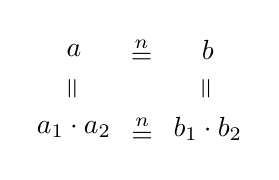
\begin{tikzpicture}[every edge/.style={draw=none}]
  \node (a) at (0, 0) {$\melt$};
  \node (b) at (1.7, 0) {$\meltB$};
  \node (b12) at (1.7, -1) {$\meltB_1 \mtimes \meltB_2$};
  \node (a12) at (0, -1) {$\melt_1 \mtimes \melt_2$};

  \path (a) edge node {$\nequiv{n}$} (b);
  \path (a12) edge node {$\nequiv{n}$} (b12);
  \path (a) edge node [rotate=90] {$=$} (a12);
  \path (b) edge node [rotate=90] {$=$} (b12);
\end{tikzpicture}\end{center}
where the $n$-equivalence at the bottom is meant to apply to the pairs of elements, \ie we demand $\melt_1 \nequiv{n} \meltB_1$ and $\melt_2 \nequiv{n} \meltB_2$.
In other words, extension carries the decomposition of $\meltB$ into $\meltB_1$ and $\meltB_2$ over the $n$-equivalence of $\melt$ and $\meltB$, and yields a corresponding decomposition of $\melt$ into $\melt_1$ and $\melt_2$.
This operation is needed to prove that $\later$ commutes with existential quantification and separating conjunction:
\begin{mathpar}
  \axiom{\later(\Exists\var:\type. \prop) \Lra \Exists\var:\type. \later\prop}
  \and\axiom{\later (\prop * \propB) \Lra \later\prop * \later\propB}
\end{mathpar}
(This assumes that the type $\type$ is non-empty.)

\begin{defn}
  An element $\munit$ of a CMRA $\monoid$ is called the \emph{unit} of $\monoid$ if it satisfies the following conditions:
  \begin{enumerate}[itemsep=0pt]
  \item $\munit$ is valid: \\ $\All n. \munit \in \mval_n$
  \item $\munit$ is a left-identity of the operation: \\
    $\All \melt \in M. \munit \mtimes \melt = \melt$
  \item $\munit$ is a discrete COFE element
  \end{enumerate}
\end{defn}

\begin{defn}
  It is possible to do a \emph{frame-preserving update} from $\melt \in \monoid$ to $\meltsB \subseteq \monoid$, written $\melt \mupd \meltsB$, if
  \[ \All n, \melt_f. \melt \mtimes \melt_f \in \mval_n \Ra \Exists \meltB \in \meltsB. \meltB \mtimes \melt_f \in \mval_n \]

  We further define $\melt \mupd \meltB \eqdef \melt \mupd \set\meltB$.
\end{defn}
Note that for RAs, this and the RA-based definition of a frame-preserving update coincide.

\begin{defn}
  A CMRA $\monoid$ is \emph{discrete} if it satisfies the following conditions:
  \begin{enumerate}[itemsep=0pt]
  \item $\monoid$ is a discrete COFE
  \item $\val$ ignores the step-index: \\
    $\All \melt \in \monoid. \melt \in \mval_0 \Ra \All n, \melt \in \mval_n$
  \end{enumerate}
\end{defn}
Note that every RA is a discrete CMRA, by picking the discrete COFE for the equivalence relation.
Furthermore, discrete CMRAs can be turned into RAs by ignoring their COFE structure, as well as the step-index of $\mval$.

\begin{defn}
  A function $f : \monoid_1 \to \monoid_2$ between two CMRAs is \emph{monotone} (written $f : \monoid_1 \monra \monoid_2$) if it satisfies the following conditions:
  \begin{enumerate}[itemsep=0pt]
  \item $f$ is non-expansive
  \item $f$ preserves validity: \\
    $\All n, \melt \in \monoid_1. \melt \in \mval_n \Ra f(\melt) \in \mval_n$
  \item $f$ preserves CMRA inclusion:\\
    $\All \melt \in \monoid_1, \meltB \in \monoid_1. \melt \mincl \meltB \Ra f(\melt) \mincl f(\meltB)$
  \end{enumerate}
\end{defn}

\begin{defn}
  The category $\CMRAs$ consists of CMRAs as objects, and monotone functions as arrows.
\end{defn}
Note that $\CMRAs$ is a subcategory of $\COFEs$.
The notion of a locally non-expansive (or contractive) bifunctor naturally generalizes to bifunctors between these categories.


%%% Local Variables: 
%%% mode: latex
%%% TeX-master: "iris"
%%% End: 

\endgroup\clearpage\begingroup
% !TEX root = ./appendix.tex
\section{COFE constructions}

\subsection{Next (type-level later)}

Given a COFE $\cofe$, we define $\latert\cofe$ as follows (using a datatype-like notation to define the type):
\begin{align*}
  \latert\cofe \eqdef{}& \latertinj(x:\cofe) \\
  \latertinj(x) \nequiv{n} \latertinj(y) \eqdef{}& n = 0 \lor x \nequiv{n-1} y
\end{align*}
Note that in the definition of the carrier $\latert\cofe$, $\latertinj$ is a constructor (like the constructors in Coq), \ie this is short for $\setComp{\latertinj(x)}{x \in \cofe}$.

$\latert(-)$ is a locally \emph{contractive} functor from $\COFEs$ to $\COFEs$.


\subsection{Uniform Predicates}

Given a CMRA $\monoid$, we define the COFE $\UPred(\monoid)$ of \emph{uniform predicates} over $\monoid$ as follows:
\begin{align*}
  \UPred(\monoid) \eqdef{} \setComp{\pred: \mathbb{N} \times \monoid \to \mProp}{
  \begin{inbox}[c]
    (\All n, x, y. \pred(n, x) \land x \nequiv{n} y \Ra \pred(n, y)) \land {}\\
    (\All n, m, x, y. \pred(n, x) \land x \mincl y \land m \leq n \land y \in \mval_m \Ra \pred(m, y))
  \end{inbox}
}
\end{align*}
where $\mProp$ is the set of meta-level propositions, \eg Coq's \texttt{Prop}.
$\UPred(-)$ is a locally non-expansive functor from $\CMRAs$ to $\COFEs$.

One way to understand this definition is to re-write it a little.
We start by defining the COFE of \emph{step-indexed propositions}: For every step-index, the proposition either holds or does not hold.
\begin{align*}
  \SProp \eqdef{}& \psetdown{\mathbb{N}} \\
    \eqdef{}& \setComp{X \in \pset{\mathbb{N}}}{ \All n, m. n \geq m \Ra n \in X \Ra m \in X } \\
  X \nequiv{n} Y \eqdef{}& \All m \leq n. m \in X \Lra m \in Y
\end{align*}
Notice that this notion of $\SProp$ is already hidden in the validity predicate $\mval_n$ of a CMRA:
We could equivalently require every CMRA to define $\mval_{-}(-) : \monoid \nfn \SProp$, replacing \ruleref{cmra-valid-ne} and \ruleref{cmra-valid-mono}.

Now we can rewrite $\UPred(\monoid)$ as monotone step-indexed predicates over $\monoid$, where the definition of a ``monotone'' function here is a little funny.
\begin{align*}
  \UPred(\monoid) \cong{}& \monoid \monra \SProp \\
     \eqdef{}& \setComp{\pred: \monoid \nfn \SProp}{\All n, m, x, y. n \in \pred(x) \land x \mincl y \land m \leq n \land y \in \mval_m \Ra m \in \pred(y)}
\end{align*}
The reason we chose the first definition is that it is easier to work with in Coq.

\clearpage
\section{RA and CMRA constructions}

\subsection{Product}
\label{sec:prodm}

Given a family $(M_i)_{i \in I}$ of CMRAs ($I$ finite), we construct a CMRA for the product $\prod_{i \in I} M_i$ by lifting everything pointwise.

Frame-preserving updates on the $M_i$ lift to the product:
\begin{mathpar}
  \inferH{prod-update}
  {\melt \mupd_{M_i} \meltsB}
  {f[i \mapsto \melt] \mupd \setComp{ f[i \mapsto \meltB]}{\meltB \in \meltsB}}
\end{mathpar}

\subsection{Sum}
\label{sec:summ}

The \emph{sum CMRA} $\monoid_1 \csumm \monoid_2$ for any CMRAs $\monoid_1$ and $\monoid_2$ is defined as (again, we use a datatype-like notation):
\begin{align*}
  \monoid_1 \csumm \monoid_2 \eqdef{}& \cinl(\melt_1:\monoid_1) \mid \cinr(\melt_2:\monoid_2) \mid \bot \\
  \mval_n \eqdef{}& \setComp{\cinl(\melt_1)\!}{\!\melt_1 \in \mval'_n}
    \cup \setComp{\cinr(\melt_2)\!}{\!\melt_2 \in \mval''_n}  \\
  \cinl(\melt_1) \mtimes \cinl(\meltB_1) \eqdef{}& \cinl(\melt_1 \mtimes \meltB_1)  \\
%  \munit \mtimes \ospending \eqdef{}& \ospending \mtimes \munit \eqdef \ospending \\
%  \munit \mtimes \osshot(\melt) \eqdef{}& \osshot(\melt) \mtimes \munit \eqdef \osshot(\melt) \\
  \mcore{\cinl(\melt_1)} \eqdef{}& \begin{cases}\mnocore & \text{if $\mcore{\melt_1} = \mnocore$} \\ \cinl({\mcore{\melt_1}}) & \text{otherwise} \end{cases}
\end{align*}
The composition and core for $\cinr$ are defined symmetrically.
The remaining cases of the composition and core are all $\bot$.
Above, $\mval'$ refers to the validity of $\monoid_1$, and $\mval''$ to the validity of $\monoid_2$.

We obtain the following frame-preserving updates, as well as their symmetric counterparts:
\begin{mathpar}
  \inferH{sum-update}
  {\melt \mupd_{M_1} \meltsB}
  {\cinl(\melt) \mupd \setComp{ \cinl(\meltB)}{\meltB \in \meltsB}}

  \inferH{sum-swap}
  {\All \melt_\f, n. \melt \mtimes \melt_\f \notin \mval'_n \and \meltB \in \mval''}
  {\cinl(\melt) \mupd \cinr(\meltB)}
\end{mathpar}
Crucially, the second rule allows us to \emph{swap} the ``side'' of the sum that the CMRA is on if $\mval$ has \emph{no possible frame}.

\subsection{Finite partial function}
\label{sec:fpfnm}

Given some infinite countable $K$ and some CMRA $\monoid$, the set of finite partial functions $K \fpfn \monoid$ is equipped with a COFE and CMRA structure by lifting everything pointwise.

We obtain the following frame-preserving updates:
\begin{mathpar}
  \inferH{fpfn-alloc-strong}
  {\text{$G$ infinite} \and \melt \in \mval}
  {\emptyset \mupd \setComp{[\gname \mapsto \melt]}{\gname \in G}}

  \inferH{fpfn-alloc}
  {\melt \in \mval}
  {\emptyset \mupd \setComp{[\gname \mapsto \melt]}{\gname \in K}}

  \inferH{fpfn-update}
  {\melt \mupd_\monoid \meltsB}
  {f[i \mapsto \melt] \mupd \setComp{ f[i \mapsto \meltB]}{\meltB \in \meltsB}}
\end{mathpar}
Above, $\mval$ refers to the validity of $\monoid$.

$K \fpfn (-)$ is a locally non-expansive functor from $\CMRAs$ to $\CMRAs$.

\subsection{Agreement}

Given some COFE $\cofe$, we define $\agm(\cofe)$ as follows:
\begin{align*}
  \agm(\cofe) \eqdef{}& \set{(c, V) \in (\mathbb{N} \to \cofe) \times \SProp}/\ {\sim} \\[-0.2em]
  \textnormal{where }& \melt \sim \meltB \eqdef{} \melt.V = \meltB.V \land 
    \All n. n \in \melt.V \Ra \melt.c(n) \nequiv{n} \meltB.c(n)  \\
%    \All n \in {\melt.V}.\, \melt.x \nequiv{n} \meltB.x \\
  \melt \nequiv{n} \meltB \eqdef{}& (\All m \leq n. m \in \melt.V \Lra m \in \meltB.V) \land (\All m \leq n. m \in \melt.V \Ra \melt.c(m) \nequiv{m} \meltB.c(m)) \\
  \mval_n \eqdef{}& \setComp{\melt \in \agm(\cofe)}{ n \in \melt.V \land \All m \leq n. \melt.c(n) \nequiv{m} \melt.c(m) } \\
  \mcore\melt \eqdef{}& \melt \\
  \melt \mtimes \meltB \eqdef{}& \left(\melt.c, \setComp{n}{n \in \melt.V \land n \in \meltB.V \land \melt \nequiv{n} \meltB }\right)
\end{align*}
%Note that the carrier $\agm(\cofe)$ is a \emph{record} consisting of the two fields $c$ and $V$.

$\agm(-)$ is a locally non-expansive functor from $\COFEs$ to $\CMRAs$.

You can think of the $c$ as a \emph{chain} of elements of $\cofe$ that has to converge only for $n \in V$ steps.
The reason we store a chain, rather than a single element, is that $\agm(\cofe)$ needs to be a COFE itself, so we need to be able to give a limit for every chain of $\agm(\cofe)$.
However, given such a chain, we cannot constructively define its limit: Clearly, the $V$ of the limit is the limit of the $V$ of the chain.
But what to pick for the actual data, for the element of $\cofe$?
Only if $V = \mathbb{N}$ we have a chain of $\cofe$ that we can take a limit of; if the $V$ is smaller, the chain ``cancels'', \ie stops converging as we reach indices $n \notin V$.
To mitigate this, we apply the usual construction to close a set; we go from elements of $\cofe$ to chains of $\cofe$.

We define an injection $\aginj$ into $\agm(\cofe)$ as follows:
\[ \aginj(x) \eqdef \record{\mathrm c \eqdef \Lam \any. x, \mathrm V \eqdef \mathbb{N}} \]
There are no interesting frame-preserving updates for $\agm(\cofe)$, but we can show the following:
\begin{mathpar}
  \axiomH{ag-val}{\aginj(x) \in \mval_n}

  \axiomH{ag-dup}{\aginj(x) = \aginj(x)\mtimes\aginj(x)}
  
  \axiomH{ag-agree}{\aginj(x) \mtimes \aginj(y) \in \mval_n \Ra x \nequiv{n} y}
\end{mathpar}


\subsection{Exclusive CMRA}

Given a COFE $\cofe$, we define a CMRA $\exm(\cofe)$ such that at most one $x \in \cofe$ can be owned:
\begin{align*}
  \exm(\cofe) \eqdef{}& \exinj(\cofe) + \bot \\
  \mval_n \eqdef{}& \setComp{\melt\in\exm(\cofe)}{\melt \neq \bot}
\end{align*}
All cases of composition go to $\bot$.
\begin{align*}
  \mcore{\exinj(x)} \eqdef{}& \mnocore &
  \mcore{\bot} \eqdef{}& \bot
\end{align*}
Remember that $\mnocore$ is the ``dummy'' element in $\maybe\monoid$ indicating (in this case) that $\exinj(x)$ has no core.

The step-indexed equivalence is inductively defined as follows:
\begin{mathpar}
  \infer{x \nequiv{n} y}{\exinj(x) \nequiv{n} \exinj(y)}

  \axiom{\bot \nequiv{n} \bot}
\end{mathpar}
$\exm(-)$ is a locally non-expansive functor from $\COFEs$ to $\CMRAs$.

We obtain the following frame-preserving update:
\begin{mathpar}
  \inferH{ex-update}{}
  {\exinj(x) \mupd \exinj(y)}
\end{mathpar}



%TODO: These need syncing with Coq
% \subsection{Finite Powerset Monoid}

% Given an infinite set $X$, we define a monoid $\textmon{PowFin}$ with carrier $\mathcal{P}^{\textrm{fin}}(X)$ as follows:
% \[
% \melt \cdot \meltB \;\eqdef\; \melt \cup \meltB \quad \mbox{if } \melt \cap \meltB = \emptyset
% \]

% We obtain:
% \begin{mathpar}
% 	\inferH{PowFinUpd}{}
% 		{\emptyset \mupd \{ \{x\} \mid x \in X  \}}
% \end{mathpar}

% \begin{proof}[Proof of \ruleref{PowFinUpd}]
% 	Assume some frame $\melt_\f \sep \emptyset$. Since $\melt_\f$ is finite and $X$ is infinite, there exists an $x \notin \melt_\f$.
% 	Pick that for the result.
% \end{proof}

% The powerset monoids is cancellative.
% \begin{proof}[Proof of cancellativity]
% 	Let $\melt_\f \mtimes \melt = \melt_\f \mtimes \meltB \neq \mzero$.
% 	So we have $\melt_\f \sep \melt$ and $\melt_\f \sep \meltB$, and we have to show $\melt = \meltB$.
% 	Assume $x \in \melt$. Hence $x \in \melt_\f \mtimes \melt$ and thus $x \in \melt_\f \mtimes \meltB$.
% 	By disjointness, $x \notin \melt_\f$ and hence $x \in meltB$.
% 	The other direction works the same way.
% \end{proof}


% \subsection{Fractional monoid}
% \label{sec:fracm}

% Given a monoid $M$, we define a monoid representing fractional ownership of some piece $\melt \in M$.
% The idea is to preserve all the frame-preserving update that $M$ could have, while additionally being able to do \emph{any} update if we own the full state (as determined by the fraction being $1$).
% Let $\fracm{M}$ be the monoid with carrier $(((0, 1] \cap \mathbb{Q}) \times M) \uplus \{\munit\}$ and multiplication
% \begin{align*}
%  (q, a) \mtimes (q', a') &\eqdef (q + q', a \mtimes a') \qquad \mbox{if $q+q'\le 1$} \\
%  (q, a) \mtimes \munit &\eqdef (q,a) \\
%  \munit \mtimes (q,a) &\eqdef (q,a).
% \end{align*}

% We get the following frame-preserving update.
% \begin{mathpar}
% 	\inferH{FracUpdFull}
% 		{a, b \in M}
% 		{(1, a) \mupd (1, b)}
%   \and\inferH{FracUpdLocal}
% 	  {a \mupd_M B}
% 	  {(q, a) \mupd \{q\} \times B}
% \end{mathpar}

% \begin{proof}[Proof of \ruleref{FracUpdFull}]
% Assume some $f \sep (1, a)$. This can only be $f = \munit$, so showing $f \sep (1, b)$ is trivial.
% \end{proof}

% \begin{proof}[Proof of \ruleref{FracUpdLocal}]
% 	Assume some $f \sep (q, a)$. If $f = \munit$, then $f \sep (q, b)$ is trivial for any $b \in B$. Just pick the one we obtain by choosing $\munit_M$ as the frame for $a$.
	
% 	In the interesting case, we have $f = (q_\f, a_\f)$.
% 	Obtain $b$ such that $b \in B \land b \sep a_\f$.
% 	Then $(q, b) \sep f$, and we are done.
% \end{proof}

% $\fracm{M}$ is cancellative if $M$ is cancellative.
% \begin{proof}[Proof of cancellativitiy]
% If $\melt_\f = \munit$, we are trivially done.
% So let $\melt_\f = (q_\f, \melt_\f')$.
% If $\melt = \munit$, then $\meltB = \munit$ as otherwise the fractions could not match up.
% Again, we are trivially done.
% Similar so for $\meltB = \munit$.
% So let $\melt = (q_a, \melt')$ and $\meltB = (q_b, \meltB')$.
% We have $(q_\f + q_a, \melt_\f' \mtimes \melt') = (q_\f + q_b, \melt_\f' \mtimes \meltB')$.
% We have to show $q_a = q_b$ and $\melt' = \meltB'$.
% The first is trivial, the second follows from cancellativitiy of $M$.
% \end{proof}


% %\subsection{Disposable monoid}
% %
% %Given a monoid $M$, we construct a monoid where, having full ownership of an element $\melt$ of $M$, one can throw it away, transitioning to a dead element.
% %Let \dispm{M} be the monoid with carrier $\mcarp{M} \uplus \{ \disposed \}$ and multiplication
% %% The previous unit must remain the unit of the new monoid, as is is always duplicable and hence we could not transition to \disposed if it were not composable with \disposed
% %\begin{align*}
% %  \melt \mtimes \meltB &\eqdef \melt \mtimes_M \meltB & \IF \melt \sep[M] \meltB \\
% %  \disposed \mtimes \disposed &\eqdef \disposed \\
% %  \munit_M \mtimes \disposed &\eqdef \disposed \mtimes \munit_M \eqdef \disposed
% %\end{align*}
% %The unit is the same as in $M$.
% %
% %The frame-preserving updates are
% %\begin{mathpar}
% % \inferH{DispUpd}
% %   {a \in \mcarp{M} \setminus \{\munit_M\} \and a \mupd_M B}
% %   {a \mupd B}
% % \and
% % \inferH{Dispose}
% %  {a \in \mcarp{M} \setminus \{\munit_M\} \and \All b \in \mcarp{M}. a \sep b \Ra b = \munit_M}
% %  {a \mupd \disposed}
% %\end{mathpar}
% %
% %\begin{proof}[Proof of \ruleref{DispUpd}]
% %Assume a frame $f$. If $f = \disposed$, then $a = \munit_M$, which is a contradiction.
% %Thus $f \in \mcarp{M}$ and we can use $a \mupd_M B$.
% %\end{proof}
% %
% %\begin{proof}[Proof of \ruleref{Dispose}]
% %The second premiss says that $a$ has no non-trivial frame in $M$. To show the update, assume a frame $f$ in $\dispm{M}$. Like above, we get $f \in \mcarp{M}$, and thus $f = \munit_M$. But $\disposed \sep \munit_M$ is trivial, so we are done.
% %\end{proof}

% \subsection{Authoritative monoid}\label{sec:auth}

% Given a monoid $M$, we construct a monoid modeling someone owning an \emph{authoritative} element $x$ of $M$, and others potentially owning fragments $\melt \le_M x$ of $x$.
% (If $M$ is an exclusive monoid, the construction is very similar to a half-ownership monoid with two asymmetric halves.)
% Let $\auth{M}$ be the monoid with carrier
% \[
% 	\setComp{ (x, \melt) }{ x \in \mcarp{\exm{\mcarp{M}}} \land \melt \in \mcarp{M} \land (x = \munit_{\exm{\mcarp{M}}} \lor \melt \leq_M x) }
% \]
% and multiplication
% \[
% (x, \melt) \mtimes (y, \meltB) \eqdef
%      (x \mtimes y, \melt \mtimes \meltB) \quad \mbox{if } x \sep y \land \melt \sep \meltB \land (x \mtimes y = \munit_{\exm{\mcarp{M}}} \lor \melt \mtimes \meltB \leq_M x \mtimes y)
% \]
% Note that $(\munit_{\exm{\mcarp{M}}}, \munit_M)$ is the unit and asserts no ownership whatsoever, but $(\munit_{M}, \munit_M)$ asserts that the authoritative element is $\munit_M$.

% Let $x, \melt \in \mcarp M$.
% We write $\authfull x$ for full ownership $(x, \munit_M):\auth{M}$ and $\authfrag \melt$ for fragmental ownership $(\munit_{\exm{\mcarp{M}}}, \melt)$ and $\authfull x , \authfrag \melt$ for combined ownership $(x, \melt)$.
% If $x$ or $a$ is $\mzero_{M}$, then the sugar denotes $\mzero_{\auth{M}}$.

% \ralf{This needs syncing with the Coq development.}
% The frame-preserving update involves a rather unwieldy side-condition:
% \begin{mathpar}
% 	\inferH{AuthUpd}{
% 		\All\melt_\f\in\mcar{\monoid}. \melt\sep\meltB \land \melt\mtimes\melt_\f \le \meltB\mtimes\melt_\f \Ra \melt'\mtimes\melt_\f \le \melt'\mtimes\meltB \and
% 		\melt' \sep \meltB
% 	}{
% 		\authfull \melt \mtimes \meltB, \authfrag \melt \mupd \authfull \melt' \mtimes \meltB, \authfrag \melt'
% 	}
% \end{mathpar}
% We therefore derive two special cases.

% \paragraph{Local frame-preserving updates.}

% \newcommand\authupd{f}%
% Following~\cite{scsl}, we say that $\authupd: \mcar{M} \ra \mcar{M}$ is \emph{local} if
% \[
% 	\All a, b \in \mcar{M}. a \sep b \land \authupd(a) \neq \mzero \Ra \authupd(a \mtimes b) = \authupd(a) \mtimes b
% \]
% Then,
% \begin{mathpar}
% 	\inferH{AuthUpdLocal}
% 	{\text{$\authupd$ local} \and \authupd(\melt)\sep\meltB}
% 	{\authfull \melt \mtimes \meltB, \authfrag \melt \mupd \authfull \authupd(\melt) \mtimes \meltB, \authfrag \authupd(\melt)}
% \end{mathpar}

% \paragraph{Frame-preserving updates on cancellative monoids.}

% Frame-preserving updates are also possible if we assume $M$ cancellative:
% \begin{mathpar}
%  \inferH{AuthUpdCancel}
%   {\text{$M$ cancellative} \and \melt'\sep\meltB}
%   {\authfull \melt \mtimes \meltB, \authfrag \melt \mupd \authfull \melt' \mtimes \meltB, \authfrag \melt'}
% \end{mathpar}

% \subsection{Fractional heap monoid}
% \label{sec:fheapm}

% By combining the fractional, finite partial function, and authoritative monoids, we construct two flavors of heaps with fractional permissions and mention their important frame-preserving updates.
% Hereinafter, we assume the set $\textdom{Val}$ of values is countable.

% Given a set $Y$, define $\FHeap(Y) \eqdef \textdom{Val} \fpfn \fracm(Y)$ representing a fractional heap with codomain $Y$.
% From \S\S\ref{sec:fracm} and~\ref{sec:fpfunm} we obtain the following frame-preserving updates as well as the fact that $\FHeap(Y)$ is cancellative.
% \begin{mathpar}
% 	\axiomH{FHeapUpd}{h[x \mapsto (1, y)] \mupd h[x \mapsto (1, y')]} \and
% 	\axiomH{FHeapAlloc}{h \mupd \{\, h[x \mapsto (1, y)] \mid x \in \textdom{Val} \,\}}
% \end{mathpar}
% We will write $qh$ with $h : \textsort{Val} \fpfn Y$ for the function in $\FHeap(Y)$ mapping every $x \in \dom(h)$ to $(q, h(x))$, and everything else to $\munit$.

% Define $\AFHeap(Y) \eqdef \auth{\FHeap(Y)}$ representing an authoritative fractional heap with codomain $Y$.
% We easily obtain the following frame-preserving updates.
% \begin{mathpar}
% 	\axiomH{AFHeapUpd}{
% 		(\authfull h[x \mapsto (1, y)], \authfrag [x \mapsto (1, y)]) \mupd (\authfull h[x \mapsto (1, y')], \authfrag [x \mapsto (1, y')])
% 	}
% 	\and
% 	\inferH{AFHeapAdd}{
% 		x \notin \dom(h)
% 	}{
% 		\authfull h \mupd (\authfull h[x \mapsto (q, y)], \authfrag [x \mapsto (q, y)])
% 	}
% 	\and
% 	\axiomH{AFHeapRemove}{
% 		(\authfull h[x \mapsto (q, y)], \authfrag [x \mapsto (q, y)]) \mupd \authfull h
% 	}
% \end{mathpar}

\subsection{STS with tokens}
\label{sec:stsmon}

Given a state-transition system~(STS, \ie a directed graph) $(\STSS, {\stsstep} \subseteq \STSS \times \STSS)$, a set of tokens $\STST$, and a labeling $\STSL: \STSS \ra \wp(\STST)$ of \emph{protocol-owned} tokens for each state, we construct an RA modeling an authoritative current state and permitting transitions given a \emph{bound} on the current state and a set of \emph{locally-owned} tokens.

The construction follows the idea of STSs as described in CaReSL \cite{caresl}.
We first lift the transition relation to $\STSS \times \wp(\STST)$ (implementing a \emph{law of token conservation}) and define a stepping relation for the \emph{frame} of a given token set:
\begin{align*}
 (s, T) \stsstep (s', T') \eqdef{}& s \stsstep s' \land \STSL(s) \uplus T = \STSL(s') \uplus T' \\
 s \stsfstep{T} s' \eqdef{}& \Exists T_1, T_2. T_1 \disj \STSL(s) \cup T \land (s, T_1) \stsstep (s', T_2)
\end{align*}

We further define \emph{closed} sets of states (given a particular set of tokens) as well as the \emph{closure} of a set:
\begin{align*}
\STSclsd(S, T) \eqdef{}& \All s \in S. \STSL(s) \disj T \land \left(\All s'. s \stsfstep{T} s' \Ra s' \in S\right) \\
\upclose(S, T) \eqdef{}& \setComp{ s' \in \STSS}{\Exists s \in S. s \stsftrans{T} s' }
\end{align*}

The STS RA is defined as follows
\begin{align*}
  \monoid \eqdef{}& \setComp{\STSauth((s, T) \in \STSS \times \wp(\STST))}{\STSL(s) \disj T} +{}\\& \setComp{\STSfrag((S, T) \in \wp(\STSS) \times \wp(\STST))}{\STSclsd(S, T) \land S \neq \emptyset} + \bot \\
  \STSfrag(S_1, T_1) \mtimes \STSfrag(S_2, T_2) \eqdef{}& \STSfrag(S_1 \cap S_2, T_1 \cup T_2) \qquad\qquad\qquad \text{if $T_1 \disj T_2$ and $S_1 \cap S_2 \neq \emptyset$} \\
  \STSfrag(S, T) \mtimes \STSauth(s, T') \eqdef{}& \STSauth(s, T') \mtimes \STSfrag(S, T) \eqdef \STSauth(s, T \cup T') \qquad \text{if $T \disj T'$ and $s \in S$} \\
  \mcore{\STSfrag(S, T)} \eqdef{}& \STSfrag(\upclose(S, \emptyset), \emptyset) \\
  \mcore{\STSauth(s, T)} \eqdef{}& \STSfrag(\upclose(\set{s}, \emptyset), \emptyset)
\end{align*}
The remaining cases are all $\bot$.

We will need the following frame-preserving update:
\begin{mathpar}
  \inferH{sts-step}{(s, T) \ststrans (s', T')}
  {\STSauth(s, T) \mupd \STSauth(s', T')}

  \inferH{sts-weaken}
  {\STSclsd(S_2, T_2) \and S_1 \subseteq S_2 \and T_2 \subseteq T_1}
  {\STSfrag(S_1, T_1) \mupd \STSfrag(S_2, T_2)}
\end{mathpar}

\paragraph{The core is not a homomorphism.}
The core of the STS construction is only satisfying the RA axioms because we are \emph{not} demanding the core to be a homomorphism---all we demand is for the core to be monotone with respect the \ruleref{ra-incl}.

In other words, the following does \emph{not} hold for the STS core as defined above:
\[ \mcore\melt \mtimes \mcore\meltB = \mcore{\melt\mtimes\meltB} \]

To see why, consider the following STS:
\newcommand\st{\textlog{s}}
\newcommand\tok{\textmon{t}}
\begin{center}
  \begin{tikzpicture}[sts]
    \node at (0,0)   (s1) {$\st_1$};
    \node at (3,0)  (s2) {$\st_2$};
    \node at (9,0) (s3) {$\st_3$};
    \node at (6,0)  (s4) {$\st_4$\\$[\tok_1, \tok_2]$};
    
    \path[sts_arrows] (s2) edge  (s4);
    \path[sts_arrows] (s3) edge  (s4);
  \end{tikzpicture}
\end{center}
Now consider the following two elements of the STS RA:
\[ \melt \eqdef \STSfrag(\set{\st_1,\st_2}, \set{\tok_1}) \qquad\qquad
  \meltB \eqdef \STSfrag(\set{\st_1,\st_3}, \set{\tok_2}) \]

We have:
\begin{mathpar}
  {\melt\mtimes\meltB = \STSfrag(\set{\st_1}, \set{\tok_1, \tok_2})}

  {\mcore\melt = \STSfrag(\set{\st_1, \st_2, \st_4}, \emptyset)}

  {\mcore\meltB = \STSfrag(\set{\st_1, \st_3, \st_4}, \emptyset)}

  {\mcore\melt \mtimes \mcore\meltB = \STSfrag(\set{\st_1, \st_4}, \emptyset) \neq
    \mcore{\melt \mtimes \meltB} = \STSfrag(\set{\st_1}, \emptyset)}
\end{mathpar}

%%% Local Variables: 
%%% mode: latex
%%% TeX-master: "iris"
%%% End: 

\endgroup\clearpage\begingroup
\section{Base Logic}
\label{sec:base-logic}

The base logic is parameterized by an arbitrary camera $\monoid$ having a unit $\munit$.
By \lemref{lem:camera-unit-total-core}, this means that the core of $\monoid$ is a total function, so we will treat it as such in the following.
This defines the structure of resources that can be owned.

As usual for higher-order logics, you can furthermore pick a \emph{signature} $\Sig = (\SigType, \SigFn, \SigAx)$ to add more types, symbols and axioms to the language.
You have to make sure that $\SigType$ includes the base types:
\[
	\SigType \supseteq \{ \textlog{M}, \Prop \}
\]
Elements of $\SigType$ are ranged over by $\sigtype$.

Each function symbol in $\SigFn$ has an associated \emph{arity} comprising a natural number $n$ and an ordered list of $n+1$ types $\type$ (the grammar of $\type$ is defined below, and depends only on $\SigType$).
We write
\[
	\sigfn : \type_1, \dots, \type_n \to \type_{n+1} \in \SigFn
\]
to express that $\sigfn$ is a function symbol with the indicated arity.

Furthermore, $\SigAx$ is a set of \emph{axioms}, that is, terms $\term$ of type $\Prop$.
Again, the grammar of terms and their typing rules are defined below, and depends only on $\SigType$ and $\SigFn$, not on $\SigAx$.
Elements of $\SigAx$ are ranged over by $\sigax$.

\subsection{Grammar}\label{sec:grammar}

\paragraph{Syntax.}
Iris syntax is built up from a signature $\Sig$ and a countably infinite set $\Var$ of variables (ranged over by metavariables $\var$, $\varB$, $\varC$).
Below, $\melt$ ranges over $\monoid$ and $i$ ranges over $\set{1,2}$.

\begin{align*}
  \type \bnfdef{}&
      \sigtype \mid
      0 \mid
      1 \mid
      \type + \type \mid
      \type \times \type \mid
      \type \to \type
\\[0.4em]
  \term, \prop, \pred \bnfdef{}&
      \var \mid
      \sigfn(\term_1, \dots, \term_n) \mid
      \textlog{abort}\; \term \mid
      () \mid
      (\term, \term) \mid
      \pi_i\; \term \mid
      \Lam \var:\type.\term \mid
      \term(\term)  \mid
\\&
      \textlog{inj}_i\; \term \mid
      \textlog{match}\; \term \;\textlog{with}\; \Ret\textlog{inj}_1\; \var. \term \mid \Ret\textlog{inj}_2\; \var. \term \;\textlog{end} \mid
%
      \melt \mid
      \mcore\term \mid
      \term \mtimes \term \mid
\\&
    \FALSE \mid
    \TRUE \mid
    \term =_\type \term \mid
    \prop \Ra \prop \mid
    \prop \land \prop \mid
    \prop \lor \prop \mid
    \prop * \prop \mid
    \prop \wand \prop \mid
\\&
    \MU \var:\type. \term  \mid
    \Exists \var:\type. \prop \mid
    \All \var:\type. \prop \mid
%\\&
    \ownM{\term} \mid \mval(\term) \mid
    \always\prop \mid
    \plainly\prop \mid
    {\later\prop} \mid
    \upd \prop
\end{align*}
Well-typedness forces recursive definitions to be \emph{guarded}:
In $\MU \var. \term$, the variable $\var$ can only appear under the later $\later$ modality.
Furthermore, the type of the definition must be \emph{complete}.
The type $\Prop$ is complete, and if $\type$ is complete, then so is $\type' \to \type$.

Note that the modalities $\upd$, $\always$, $\plainly$ and $\later$ bind more tightly than $*$, $\wand$, $\land$, $\lor$, and $\Ra$.


\paragraph{Variable conventions.}
We assume that, if a term occurs multiple times in a rule, its free variables are exactly those binders which are available at every occurrence.


\subsection{Types}\label{sec:types}

Iris terms are simply-typed.
The judgment $\vctx \proves \wtt{\term}{\type}$ expresses that, in variable context $\vctx$, the term $\term$ has type $\type$.

A variable context, $\vctx = x_1:\type_1, \dots, x_n:\type_n$, declares a list of variables and their types.
In writing $\vctx, x:\type$, we presuppose that $x$ is not already declared in $\vctx$.

\judgment[Well-typed terms]{\vctx \proves_\Sig \wtt{\term}{\type}}
\begin{mathparpagebreakable}
%%% variables and function symbols
	\axiom{x : \type \proves \wtt{x}{\type}}
\and
	\infer{\vctx \proves \wtt{\term}{\type}}
		{\vctx, x:\type' \proves \wtt{\term}{\type}}
\and
	\infer{\vctx, x:\type', y:\type' \proves \wtt{\term}{\type}}
		{\vctx, x:\type' \proves \wtt{\term[x/y]}{\type}}
\and
	\infer{\vctx_1, x:\type', y:\type'', \vctx_2 \proves \wtt{\term}{\type}}
		{\vctx_1, x:\type'', y:\type', \vctx_2 \proves \wtt{\term[y/x,x/y]}{\type}}
\and
	\infer{
		\vctx \proves \wtt{\term_1}{\type_1} \and
		\cdots \and
		\vctx \proves \wtt{\term_n}{\type_n} \and
		\sigfn : \type_1, \dots, \type_n \to \type_{n+1} \in \SigFn
	}{
		\vctx \proves \wtt {\sigfn(\term_1, \dots, \term_n)} {\type_{n+1}}
	}
%%% empty, unit, products, sums
\and
	\infer{\vctx \proves \wtt\term{0}}
        {\vctx \proves \wtt{\textlog{abort}\; \term}\type}
\and
	\axiom{\vctx \proves \wtt{()}{1}}
\and
	\infer{\vctx \proves \wtt{\term}{\type_1} \and \vctx \proves \wtt{\termB}{\type_2}}
		{\vctx \proves \wtt{(\term,\termB)}{\type_1 \times \type_2}}
\and
	\infer{\vctx \proves \wtt{\term}{\type_1 \times \type_2} \and i \in \{1, 2\}}
		{\vctx \proves \wtt{\pi_i\,\term}{\type_i}}
\and
        \infer{\vctx \proves \wtt\term{\type_i} \and i \in \{1, 2\}}
        {\vctx \proves \wtt{\textlog{inj}_i\;\term}{\type_1 + \type_2}}
\and
        \infer{\vctx \proves \wtt\term{\type_1 + \type_2} \and
        \vctx, \var:\type_1 \proves \wtt{\term_1}\type \and
        \vctx, \varB:\type_2 \proves \wtt{\term_2}\type}
        {\vctx \proves \wtt{\textlog{match}\; \term \;\textlog{with}\; \Ret\textlog{inj}_1\; \var. \term_1 \mid \Ret\textlog{inj}_2\; \varB. \term_2 \;\textlog{end}}{\type}}
%%% functions
\and
	\infer{\vctx, x:\type \proves \wtt{\term}{\type'}}
		{\vctx \proves \wtt{\Lam x. \term}{\type \to \type'}}
\and
	\infer
	{\vctx \proves \wtt{\term}{\type \to \type'} \and \wtt{\termB}{\type}}
	{\vctx \proves \wtt{\term(\termB)}{\type'}}
%%% monoids
\and
        \infer{}{\vctx \proves \wtt\melt{\textlog{M}}}
\and
	\infer{\vctx \proves \wtt\melt{\textlog{M}}}{\vctx \proves \wtt{\mcore\melt}{\textlog{M}}}
\and
	\infer{\vctx \proves \wtt{\melt}{\textlog{M}} \and \vctx \proves \wtt{\meltB}{\textlog{M}}}
		{\vctx \proves \wtt{\melt \mtimes \meltB}{\textlog{M}}}
%%% props and predicates
\\
	\axiom{\vctx \proves \wtt{\FALSE}{\Prop}}
\and
	\axiom{\vctx \proves \wtt{\TRUE}{\Prop}}
\and
	\infer{\vctx \proves \wtt{\term}{\type} \and \vctx \proves \wtt{\termB}{\type}}
		{\vctx \proves \wtt{\term =_\type \termB}{\Prop}}
\and
	\infer{\vctx \proves \wtt{\prop}{\Prop} \and \vctx \proves \wtt{\propB}{\Prop}}
		{\vctx \proves \wtt{\prop \Ra \propB}{\Prop}}
\and
	\infer{\vctx \proves \wtt{\prop}{\Prop} \and \vctx \proves \wtt{\propB}{\Prop}}
		{\vctx \proves \wtt{\prop \land \propB}{\Prop}}
\and
	\infer{\vctx \proves \wtt{\prop}{\Prop} \and \vctx \proves \wtt{\propB}{\Prop}}
		{\vctx \proves \wtt{\prop \lor \propB}{\Prop}}
\and
	\infer{\vctx \proves \wtt{\prop}{\Prop} \and \vctx \proves \wtt{\propB}{\Prop}}
		{\vctx \proves \wtt{\prop * \propB}{\Prop}}
\and
	\infer{\vctx \proves \wtt{\prop}{\Prop} \and \vctx \proves \wtt{\propB}{\Prop}}
		{\vctx \proves \wtt{\prop \wand \propB}{\Prop}}
\and
	\infer{
		\vctx, \var:\type \proves \wtt{\term}{\type} \and
		\text{$\var$ is guarded in $\term$} \and
		\text{$\type$ is complete}
	}{
		\vctx \proves \wtt{\MU \var:\type. \term}{\type}
	}
\and
	\infer{\vctx, x:\type \proves \wtt{\prop}{\Prop}}
		{\vctx \proves \wtt{\Exists x:\type. \prop}{\Prop}}
\and
	\infer{\vctx, x:\type \proves \wtt{\prop}{\Prop}}
		{\vctx \proves \wtt{\All x:\type. \prop}{\Prop}}
\and
	\infer{\vctx \proves \wtt{\melt}{\textlog{M}}}
		{\vctx \proves \wtt{\ownM{\melt}}{\Prop}}
\and
	\infer{\vctx \proves \wtt{\melt}{\type} \and \text{$\type$ is a camera}}
		{\vctx \proves \wtt{\mval(\melt)}{\Prop}}
\and
	\infer{\vctx \proves \wtt{\prop}{\Prop}}
		{\vctx \proves \wtt{\always\prop}{\Prop}}
\and
	\infer{\vctx \proves \wtt{\prop}{\Prop}}
		{\vctx \proves \wtt{\plainly\prop}{\Prop}}
\and
	\infer{\vctx \proves \wtt{\prop}{\Prop}}
		{\vctx \proves \wtt{\later\prop}{\Prop}}
\and
	\infer{
		\vctx \proves \wtt{\prop}{\Prop}
	}{
		\vctx \proves \wtt{\upd \prop}{\Prop}
	}
\end{mathparpagebreakable}

\subsection{Proof Rules}
\label{sec:proof-rules}

The judgment $\vctx \mid \prop \proves \propB$ says that with free variables $\vctx$, proposition $\propB$ holds whenever assumption $\prop$ holds.
Most of the rules will entirely omit the variable contexts $\vctx$.
In this case, we assume the same arbitrary context is used for every constituent of the rules.
%Furthermore, an arbitrary \emph{boxed} assertion context $\always\pfctx$ may be added to every constituent.
Axioms $\vctx \mid \prop \provesIff \propB$ indicate that both $\vctx \mid \prop \proves \propB$ and $\vctx \mid \propB \proves \prop$ are proof rules of the logic.

\judgment{\vctx \mid \prop \proves \propB}
\paragraph{Laws of intuitionistic higher-order logic with equality.}
This is entirely standard.
\begin{mathparpagebreakable}
\infer[Asm]
  {}
  {\prop \proves \prop}
\and
\infer[Cut]
  {\prop \proves \propB \and \propB \proves \propC}
  {\prop \proves \propC}
\and
\infer[Eq]
  {\vctx,\var:\type \proves \wtt\propB\Prop \\ \vctx\mid\prop \proves \propB[\term/\var] \\ \vctx\mid\prop \proves \term =_\type \term'}
  {\vctx\mid\prop \proves \propB[\term'/\var]}
\and
\infer[Refl]
  {}
  {\TRUE \proves \term =_\type \term}
\and
\infer[$\bot$E]
  {}
  {\FALSE \proves \prop}
\and
\infer[$\top$I]
  {}
  {\prop \proves \TRUE}
\and
\infer[$\wedge$I]
  {\prop \proves \propB \\ \prop \proves \propC}
  {\prop \proves \propB \land \propC}
\and
\infer[$\wedge$EL]
  {\prop \proves \propB \land \propC}
  {\prop \proves \propB}
\and
\infer[$\wedge$ER]
  {\prop \proves \propB \land \propC}
  {\prop \proves \propC}
\and
\infer[$\vee$IL]
  {\prop \proves \propB }
  {\prop \proves \propB \lor \propC}
\and
\infer[$\vee$IR]
  {\prop \proves \propC}
  {\prop \proves \propB \lor \propC}
\and
\infer[$\vee$E]
  {\prop \proves \propC \\
   \propB \proves \propC}
  {\prop \lor \propB \proves \propC}
\and
\infer[$\Ra$I]
  {\prop \land \propB \proves \propC}
  {\prop \proves \propB \Ra \propC}
\and
\infer[$\Ra$E]
  {\prop \proves \propB \Ra \propC \\ \prop \proves \propB}
  {\prop \proves \propC}
\and
\infer[$\forall$I]
  { \vctx,\var : \type\mid\prop \proves \propB}
  {\vctx\mid\prop \proves \All \var: \type. \propB}
\and
\infer[$\forall$E]
  {\vctx\mid\prop \proves \All \var :\type. \propB \\
   \vctx \proves \wtt\term\type}
  {\vctx\mid\prop \proves \propB[\term/\var]}
\\
\infer[$\exists$I]
  {\vctx\mid\prop \proves \propB[\term/\var] \\
   \vctx \proves \wtt\term\type}
  {\vctx\mid\prop \proves \exists \var: \type. \propB}
\and
\infer[$\exists$E]
  {\vctx,\var : \type\mid\prop \proves \propB}
  {\vctx\mid\Exists \var: \type. \prop \proves \propB}
% \and
% \infer[$\lambda$]
%   {}
%   {\pfctx \proves (\Lam\var: \type. \prop)(\term) =_{\type\to\type'} \prop[\term/\var]}
% \and
% \infer[$\mu$]
%   {}
%   {\pfctx \proves \mu\var: \type. \prop =_{\type} \prop[\mu\var: \type. \prop/\var]}
\end{mathparpagebreakable}
Furthermore, we have the usual $\eta$ and $\beta$ laws for projections, $\textlog{abort}$, sum elimination, $\lambda$ and $\mu$.


\paragraph{Laws of (affine) bunched implications.}
\begin{mathpar}
\begin{array}{rMcMl}
  \TRUE * \prop &\provesIff& \prop \\
  \prop * \propB &\proves& \propB * \prop \\
  (\prop * \propB) * \propC &\proves& \prop * (\propB * \propC)
\end{array}
\and
\infer[$*$-mono]
  {\prop_1 \proves \propB_1 \and
   \prop_2 \proves \propB_2}
  {\prop_1 * \prop_2 \proves \propB_1 * \propB_2}
\and
\inferB[$\wand$I-E]
  {\prop * \propB \proves \propC}
  {\prop \proves \propB \wand \propC}
\end{mathpar}

\paragraph{Laws for the plainness modality.}
\begin{mathpar}
\infer[$\plainly$-mono]
  {\prop \proves \propB}
  {\plainly{\prop} \proves \plainly{\propB}}
\and
\infer[$\plainly$-E]{}
{\plainly\prop \proves \always\prop}
\and
\begin{array}[c]{rMcMl}
  (\plainly P \Ra \plainly Q) &\proves& \plainly (\plainly P \Ra Q) \\
\plainly ( ( P \Ra Q) \land (Q \Ra P ) ) &\proves& P =_{\Prop} Q
\end{array}
\and
\begin{array}[c]{rMcMl}
  \plainly{\prop} &\proves& \plainly\plainly\prop \\
  \All x. \plainly{\prop} &\proves& \plainly{\All x. \prop} \\
  \plainly{\Exists x. \prop} &\proves& \Exists x. \plainly{\prop}
\end{array}
%\and
%\infer[PropExt]{}{\plainly ( ( P \Ra Q) \land (Q \Ra P ) ) \proves P =_{\Prop} Q}
\end{mathpar}

\paragraph{Laws for the persistence modality.}
\begin{mathpar}
\infer[$\always$-mono]
  {\prop \proves \propB}
  {\always{\prop} \proves \always{\propB}}
\and
\infer[$\always$-E]{}
{\always\prop \proves \prop}
\and
\begin{array}[c]{rMcMl}
  (\plainly P \Ra \always Q) &\proves& \always (\plainly P \Ra Q) \\
  \always{\prop} \land \propB &\proves& \always{\prop} * \propB
\end{array}
\and
\begin{array}[c]{rMcMl}
  \always{\prop} &\proves& \always\always\prop \\
  \All x. \always{\prop} &\proves& \always{\All x. \prop} \\
  \always{\Exists x. \prop} &\proves& \Exists x. \always{\prop}
\end{array}
\end{mathpar}


\paragraph{Laws for the later modality.}
\begin{mathpar}
\infer[$\later$-mono]
  {\prop \proves \propB}
  {\later\prop \proves \later{\propB}}
\and
\inferhref{L{\"o}b}{Loeb}
  {}
  {(\later\prop\Ra\prop) \proves \prop}
\and
\begin{array}[c]{rMcMl}
  \All x. \later\prop &\proves& \later{\All x.\prop} \\
  \later\Exists x. \prop &\proves& \later\FALSE \lor {\Exists x.\later\prop}  \\
  \later\prop &\proves& \later\FALSE \lor (\later\FALSE \Ra \prop)
\end{array}
\and
\begin{array}[c]{rMcMl}
  \later{(\prop * \propB)} &\provesIff& \later\prop * \later\propB \\
  \always{\later\prop} &\provesIff& \later\always{\prop} \\
  \plainly{\later\prop} &\provesIff& \later\plainly{\prop}
\end{array}
\end{mathpar}


\paragraph{Laws for resources and validity.}
\begin{mathpar}
\begin{array}{rMcMl}
\ownM{\melt} * \ownM{\meltB} &\provesIff&  \ownM{\melt \mtimes \meltB} \\
\ownM\melt &\proves& \always{\ownM{\mcore\melt}} \\
\TRUE &\proves&  \ownM{\munit} \\
\later\ownM\melt &\proves& \Exists\meltB. \ownM\meltB \land \later(\melt = \meltB)
\end{array}
% \and
% \infer[valid-intro]
% {\melt \in \mval}
% {\TRUE \vdash \mval(\melt)}
% \and
% \infer[valid-elim]
% {\melt \notin \mval_0}
% {\mval(\melt) \proves \FALSE}
\and
\begin{array}{rMcMl}
\ownM{\melt} &\proves& \mval(\melt) \\
\mval(\melt \mtimes \meltB) &\proves& \mval(\melt) \\
\mval(\melt) &\proves& \always\mval(\melt)
\end{array}
\end{mathpar}


\paragraph{Laws for the basic update modality.}
\begin{mathpar}
\inferH{upd-mono}
{\prop \proves \propB}
{\upd\prop \proves \upd\propB}

\inferH{upd-intro}
{}{\prop \proves \upd \prop}

\inferH{upd-trans}
{}
{\upd \upd \prop \proves \upd \prop}

\inferH{upd-frame}
{}{\propB * \upd\prop \proves \upd (\propB * \prop)}

\inferH{upd-update}
{\melt \mupd \meltsB}
{\ownM\melt \proves \upd \Exists\meltB\in\meltsB. \ownM\meltB}

\inferH{upd-plainly}
{}
{\upd\plainly\prop \proves \prop}
\end{mathpar}
The premise in \ruleref{upd-update} is a \emph{meta-level} side-condition that has to be proven about $a$ and $B$.
%\ralf{Trouble is, we don't actually have $\in$ inside the logic...}

\subsection{Consistency}

The consistency statement of the logic reads as follows: For any $n$, we have
\begin{align*}
  \lnot(\TRUE \proves (\later)^n\spac\FALSE)
\end{align*}
where $(\later)^n$ is short for $\later$ being nested $n$ times.

The reason we want a stronger consistency than the usual $\lnot(\TRUE \proves \FALSE)$ is our modalities: it should be impossible to derive a contradiction below the modalities.
For $\always$ and $\plainly$, this follows from the elimination rules.
For updates, we use the fact that $\upd\FALSE \proves \upd\plainly\FALSE \proves \FALSE$.
However, there is no elimination rule for $\later$, so we declare that it is impossible to derive a contradiction below any number of laters.


%%% Local Variables:
%%% mode: latex
%%% TeX-master: "iris"
%%% End:

\endgroup\clearpage\begingroup
\section{Model and semantics}
\label{sec:model}

The semantics closely follows the ideas laid out in~\cite{catlogic}.

\paragraph{Semantic domains.}

The semantic  domains are interpreted as follows:
\[
\begin{array}[t]{@{}l@{\ }c@{\ }l@{}}
\Sem{\textlog{\Prop}} &\eqdef& \UPred(\monoid)  \\
\Sem{\textlog{M}} &\eqdef& \monoid
\end{array}
\qquad\qquad
\begin{array}[t]{@{}l@{\ }c@{\ }l@{}}
\Sem{1} &\eqdef& \Delta \{ () \} \\
\Sem{\type \times \type'} &\eqdef& \Sem{\type} \times \Sem{\type} \\
\Sem{\type \to \type'} &\eqdef& \Sem{\type} \nfn \Sem{\type} \\
\end{array}
\]
For the remaining base types $\type$ defined by the signature $\Sig$, we pick an object $X_\type$ in $\COFEs$ and define
\[
\Sem{\type} \eqdef X_\type
\]
For each function symbol $\sigfn : \type_1, \dots, \type_n \to \type_{n+1} \in \SigFn$, we pick a function $\Sem{\sigfn} : \Sem{\type_1} \times \dots \times \Sem{\type_n} \nfn \Sem{\type_{n+1}}$.

\judgment[Interpretation of assertions.]{\Sem{\vctx \proves \term : \Prop} : \Sem{\vctx} \nfn \UPred(\monoid)}

Remember that $\UPred(\monoid)$ is isomorphic to $\monoid \monra \SProp$.
We are thus going to define the assertions as mapping CMRA elements to sets of step-indices.

\begin{align*}
	\Sem{\vctx \proves t =_\type u : \Prop}_\gamma &\eqdef
	\Lam \any. \setComp{n}{\Sem{\vctx \proves t : \type}_\gamma \nequiv{n} \Sem{\vctx \proves u : \type}_\gamma} \\
	\Sem{\vctx \proves \FALSE : \Prop}_\gamma &\eqdef \Lam \any. \emptyset \\
	\Sem{\vctx \proves \TRUE : \Prop}_\gamma &\eqdef \Lam \any. \mathbb{N} \\
	\Sem{\vctx \proves \prop \land \propB : \Prop}_\gamma &\eqdef
	\Lam \melt. \Sem{\vctx \proves \prop : \Prop}_\gamma(\melt) \cap \Sem{\vctx \proves \propB : \Prop}_\gamma(\melt) \\
	\Sem{\vctx \proves \prop \lor \propB : \Prop}_\gamma &\eqdef
	\Lam \melt. \Sem{\vctx \proves \prop : \Prop}_\gamma(\melt) \cup \Sem{\vctx \proves \propB : \Prop}_\gamma(\melt) \\
	\Sem{\vctx \proves \prop \Ra \propB : \Prop}_\gamma &\eqdef
	\Lam \melt. \setComp{n}{\begin{aligned}
            \All m, \meltB.& m \leq n \land \melt \mincl \meltB \land \meltB \in \mval_m \Ra {} \\
            & m \in \Sem{\vctx \proves \prop : \Prop}_\gamma(\meltB) \Ra {}\\& m \in \Sem{\vctx \proves \propB : \Prop}_\gamma(\meltB)\end{aligned}}\\
	\Sem{\vctx \proves \All \var : \type. \prop : \Prop}_\gamma &\eqdef
	\Lam \melt. \setComp{n}{ \All v \in \Sem{\type}. n \in \Sem{\vctx, \var : \type \proves \prop : \Prop}_{\mapinsert \var v \gamma}(\melt) } \\
	\Sem{\vctx \proves \Exists \var : \type. \prop : \Prop}_\gamma &\eqdef
        \Lam \melt. \setComp{n}{ \Exists v \in \Sem{\type}. n \in \Sem{\vctx, \var : \type \proves \prop : \Prop}_{\mapinsert \var v \gamma}(\melt) } \\
  ~\\
	\Sem{\vctx \proves \prop * \propB : \Prop}_\gamma &\eqdef \Lam\melt. \setComp{n}{\begin{aligned}\Exists \meltB_1, \meltB_2. &\melt \nequiv{n} \meltB_1 \mtimes \meltB_2 \land {}\\& n \in \Sem{\vctx \proves \prop : \Prop}_\gamma(\meltB_1) \land n \in \Sem{\vctx \proves \propB : \Prop}_\gamma(\meltB_2)\end{aligned}}
\\
	\Sem{\vctx \proves \prop \wand \propB : \Prop}_\gamma &\eqdef
	\Lam \melt. \setComp{n}{\begin{aligned}
            \All m, \meltB.& m \leq n \land  \melt\mtimes\meltB \in \mval_m \Ra {} \\
            & m \in \Sem{\vctx \proves \prop : \Prop}_\gamma(\meltB) \Ra {}\\& m \in \Sem{\vctx \proves \propB : \Prop}_\gamma(\melt\mtimes\meltB)\end{aligned}} \\
	\Sem{\vctx \proves \always{\prop} : \Prop}_\gamma &\eqdef \Lam\melt. \Sem{\vctx \proves \prop : \Prop}_\gamma(\mcore\melt) \\
	\Sem{\vctx \proves \later{\prop} : \Prop}_\gamma &\eqdef \Lam\melt. \setComp{n}{n = 0 \lor n-1 \in \Sem{\vctx \proves \prop : \Prop}_\gamma(\melt)}\\
        \Sem{\vctx \proves \ownM{\melt} : \Prop}_\gamma &\eqdef \Lam\meltB. \setComp{n}{\Sem{\vctx \proves \melt : \textlog{M}}_\gamma \mincl[n] \meltB}  \\
        \Sem{\vctx \proves \mval(\melt) : \Prop}_\gamma &\eqdef \Lam\any. \setComp{n}{\Sem{\vctx \proves \melt : \type}_\gamma \in \mval_n} \\
        \Sem{\vctx \proves \upd\prop : \Prop}_\gamma &\eqdef \Lam\melt. \setComp{n}{\begin{aligned}
            \All m, \melt'. & m \leq n \land (\melt \mtimes \melt') \in \mval_m \Ra {}\\& \Exists \meltB. (\meltB \mtimes \melt') \in \mval_m \land m \in \Sem{\vctx \proves \prop :\Prop}_\gamma(\meltB)
          \end{aligned}
}
\end{align*}

For every definition, we have to show all the side-conditions: The maps have to be non-expansive and monotone.



\judgment[Interpretation of non-propositional terms]{\Sem{\vctx \proves \term : \type} : \Sem{\vctx} \nfn \Sem{\type}}
\begin{align*}
	\Sem{\vctx \proves x : \type}_\gamma &\eqdef \gamma(x) \\
	\Sem{\vctx \proves \sigfn(\term_1, \dots, \term_n) : \type_{n+1}}_\gamma &\eqdef \Sem{\sigfn}(\Sem{\vctx \proves \term_1 : \type_1}_\gamma, \dots, \Sem{\vctx \proves \term_n : \type_n}_\gamma) \\
	\Sem{\vctx \proves \Lam \var:\type. \term : \type \to \type'}_\gamma &\eqdef
	\Lam \termB : \Sem{\type}. \Sem{\vctx, \var : \type \proves \term : \type}_{\mapinsert \var \termB \gamma]} \\
	\Sem{\vctx \proves \term(\termB) : \type'}_\gamma &\eqdef
	\Sem{\vctx \proves \term : \type \to \type'}_\gamma(\Sem{\vctx \proves \termB : \type}_\gamma) \\
	\Sem{\vctx \proves \MU \var:\type. \term : \type}_\gamma &\eqdef
	\mathit{fix}(\Lam \termB : \Sem{\type}. \Sem{\vctx, x : \type \proves \term : \type}_{\mapinsert \var \termB \gamma}) \\
  ~\\
	\Sem{\vctx \proves () : 1}_\gamma &\eqdef () \\
	\Sem{\vctx \proves (\term_1, \term_2) : \type_1 \times \type_2}_\gamma &\eqdef (\Sem{\vctx \proves \term_1 : \type_1}_\gamma, \Sem{\vctx \proves \term_2 : \type_2}_\gamma) \\
	\Sem{\vctx \proves \pi_i(\term) : \type_i}_\gamma &\eqdef \pi_i(\Sem{\vctx \proves \term : \type_1 \times \type_2}_\gamma) \\
  ~\\
	\Sem{\vctx \proves \mcore\melt : \textlog{M}}_\gamma &\eqdef \mcore{\Sem{\vctx \proves \melt : \textlog{M}}_\gamma} \\
	\Sem{\vctx \proves \melt \mtimes \meltB : \textlog{M}}_\gamma &\eqdef
	\Sem{\vctx \proves \melt : \textlog{M}}_\gamma \mtimes \Sem{\vctx \proves \meltB : \textlog{M}}_\gamma
\end{align*}
%

An environment $\vctx$ is interpreted as the set of
finite partial functions $\rho$, with $\dom(\rho) = \dom(\vctx)$ and
$\rho(x)\in\Sem{\vctx(x)}$.

\paragraph{Logical entailment.}
We can now define \emph{semantic} logical entailment.

\typedsection{Interpretation of entailment}{\Sem{\vctx \mid \pfctx \proves \prop} : \mProp}

\[
\Sem{\vctx \mid \prop \proves \propB} \eqdef
\begin{aligned}[t]
\MoveEqLeft
\forall n \in \mathbb{N}.\;
\forall \rs \in \textdom{Res}.\; 
\forall \gamma \in \Sem{\vctx},\;
\\&
n \in \Sem{\vctx \proves \prop : \Prop}_\gamma(\rs)
\Ra n \in \Sem{\vctx \proves \propB : \Prop}_\gamma(\rs)
\end{aligned}
\]

The following soundness theorem connects syntactic and semantic entailment.
It is proven by showing that all the syntactic proof rules of \Sref{sec:base-logic} can be validated in the model.
\[ \vctx \mid \prop \proves \propB \Ra \Sem{\vctx \mid \prop \proves \propB} \]

It now becomes straight-forward to show consistency of the logic.

%%% Local Variables:
%%% mode: latex
%%% TeX-master: "iris"
%%% End:

\endgroup\clearpage\begingroup
\section{Modular Dynamic Higher-Order Resources}
\label{sec:hogs}

The logic described in \Sref{sec:base-logic} works over an arbitrary CMRA $\monoid$ defining the structure of the resources.
It turns out that we can generalize this further and permit picking CMRAs ``$\iFunc(\Prop)$'' that depend on the structure of assertions themselves.
Of course, $\Prop$ is just the syntactic type of assertions; for this to make sense we have to look at the semantics.

To instantiate the logic, you pick a family of locally contractive bifunctors $(\iFunc_i : \COFEs \to \CMRAs)_{i \in \mathcal{I}}$.

From this, we construct the bifunctor defining the overall resources as follows:
\begin{align*}
  \textdom{ResF}(\cofe^\op, \cofe) \eqdef{}& \prod_{i \in \mathcal I} \mathbb{N} \fpfn \iFunc_i(\cofe^\op, \cofe)
\end{align*}
$\textdom{ResF}(\cofe^\op, \cofe)$ is a CMRA by lifting the individual CMRAs pointwise, and it has a unit (using the empty finite partial functions).
Furthermore, since the $\iFunc_i$ are locally contractive, so is $\textdom{ResF}$.

Now we can write down the recursive domain equation:
\[ \iPreProp \cong \UPred(\textdom{ResF}(\iPreProp, \iPreProp)) \]
$\iPreProp$ is a COFE defined as the fixed-point of a locally contractive bifunctor.
This fixed-point exists and is unique by America and Rutten's theorem~\cite{America-Rutten:JCSS89,birkedal:metric-space}.
We do not need to consider how the object is constructed. 
We only need the isomorphism, given by
\begin{align*}
  \Res &\eqdef \textdom{ResF}(\iPreProp, \iPreProp) \\
  \iProp &\eqdef \UPred(\Res) \\
	\wIso &: \iProp \nfn \iPreProp \\
	\wIso^{-1} &: \iPreProp \nfn \iProp
\end{align*}

Notice that $\iProp$ is the semantic model of assertions for  the logic described in \Sref{sec:base-logic} with $\Res$:
\[ \Sem{\Prop} \eqdef \iProp = \UPred(\Res) \]
We thus obtain all the rules of \Sref{sec:base-logic}, and furthermore, we can use the maps $\wIso$ and $\wIso^{-1}$ \emph{in the logic} to convert between logical assertions and the domain $\iPreProp$ which is used in the construction of $\Res$ -- so from elements of $\iPreProp$, we can construct elements of $\Sem{\textlog M}$, which are the elements that can be owned in our logic.

\ralf{TODO: Describe the pattern of only assuming some elements of the index family to indicate a particular functor.}
\ralf{TODO: Show the rules for ownership in this world.}




%%% Local Variables:
%%% mode: latex
%%% TeX-master: "iris"
%%% End:

\endgroup\clearpage\begingroup
\section{Language}
\label{sec:language}

A \emph{language} $\Lang$ consists of a set \Expr{} of \emph{expressions} (metavariable $\expr$), a set \Val{} of \emph{values} (metavariable $\val$), and a nonempty set $\State$ of \emph{states} (metavariable $\state$) such that
\begin{itemize}[itemsep=0pt]
\item There exist functions $\ofval : \Val \to \Expr$ and $\toval : \Expr \pfn \Val$ (notice the latter is partial), such that
\begin{mathpar}
{\All \expr, \val. \toval(\expr) = \val \Ra \ofval(\val) = \expr} \and
{\All\val. \toval(\ofval(\val)) = \val} 
\end{mathpar}
\item There exists a \emph{primitive reduction relation} \[(-,- \step -,-,-) \subseteq \Expr \times \State \times \Expr \times \State \times \List(\Expr)\]
  A reduction $\expr_1, \state_1 \step \expr_2, \state_2, \overline\expr$ indicates that, when $\expr_1$ reduces to $\expr_2$, the new threads in the list $\overline\expr$ is forked off.
  We will write $\expr_1, \state_1 \step \expr_2, \state_2$ for $\expr_1, \state_1 \step \expr_2, \state_2, ()$, \ie when no threads are forked off. \\
\item All values are stuck:
\[ \expr, \_ \step  \_, \_, \_ \Ra \toval(\expr) = \bot \]
\end{itemize}

\begin{defn}
  An expression $\expr$ and state $\state$ are \emph{reducible} (written $\red(\expr, \state)$) if
  \[ \Exists \expr_2, \state_2, \vec\expr. \expr,\state \step \expr_2,\state_2,\vec\expr \]
\end{defn}

\begin{defn}
  An expression $\expr$ is \emph{weakly atomic} if it reduces in one step to something irreducible:
  \[ \atomic(\expr) \eqdef \All\state_1, \expr_2, \state_2, \vec\expr. \expr, \state_1 \step \expr_2, \state_2, \vec\expr \Ra \lnot \red(\expr_2, \state_2) \]
  It is \emph{strongly atomic} if it reduces in one step to a value:
  \[ \stronglyAtomic(\expr) \eqdef \All\state_1, \expr_2, \state_2, \vec\expr. \expr, \state_1 \step \expr_2, \state_2, \vec\expr \Ra \toval(\expr_2) \neq \bot \]
\end{defn}
We need two notions of atomicity to accommodate both kinds of weakest preconditions that we will define later:
If the weakest precondition ensures that the program cannot get stuck, weak atomicity is sufficient.
Otherwise, we need strong atomicity.

\begin{defn}[Context]
  A function $\lctx : \Expr \to \Expr$ is a \emph{context} if the following conditions are satisfied:
  \begin{enumerate}[itemsep=0pt]
  \item $\lctx$ does not turn non-values into values:\\
    $\All\expr. \toval(\expr) = \bot \Ra \toval(\lctx(\expr)) = \bot $
  \item One can perform reductions below $\lctx$:\\
    $\All \expr_1, \state_1, \expr_2, \state_2, \vec\expr. \expr_1, \state_1 \step \expr_2,\state_2,\vec\expr \Ra \lctx(\expr_1), \state_1 \step \lctx(\expr_2),\state_2,\vec\expr $
  \item Reductions stay below $\lctx$ until there is a value in the hole:\\
    $\All \expr_1', \state_1, \expr_2, \state_2, \vec\expr. \toval(\expr_1') = \bot \land \lctx(\expr_1'), \state_1 \step \expr_2,\state_2,\vec\expr \Ra \Exists\expr_2'. \expr_2 = \lctx(\expr_2') \land \expr_1', \state_1 \step \expr_2',\state_2,\vec\expr $
  \end{enumerate}
\end{defn}

\subsection{Concurrent Language}

For any language $\Lang$, we define the corresponding thread-pool semantics.

\paragraph{Machine syntax}
\[
	\tpool \in \ThreadPool \eqdef \List(\Expr)
\]

\judgment[Machine reduction]{\cfg{\tpool}{\state} \step
  \cfg{\tpool'}{\state'}}
\begin{mathpar}
\infer
  {\expr_1, \state_1 \step \expr_2, \state_2, \vec\expr}
  {\cfg{\tpool \dplus [\expr_1] \dplus \tpool'}{\state_1} \step
     \cfg{\tpool \dplus [\expr_2] \dplus \tpool' \dplus \vec\expr}{\state_2}}
\end{mathpar}


%%% Local Variables:
%%% mode: latex
%%% TeX-master: "iris"
%%% End:

\endgroup\clearpage\begingroup
\let\bar\overline

\section{Language}
\label{sec:language}

A \emph{language} $\Lang$ consists of a set \textdom{Expr} of \emph{expressions} (metavariable $\expr$), a set \textdom{Val} of \emph{values} (metavariable $\val$), and a set \textdom{State} of \emph{states} (metvariable $\state$) such that
\begin{itemize}
\item There exist functions $\ofval : \textdom{Val} \to \textdom{Expr}$ and $\toval : \textdom{Expr} \pfn \textdom{val}$ (notice the latter is partial), such that
\begin{mathpar} {\All \expr, \val. \toval(\expr) = \val \Ra \ofval(\val) = \expr} \and {\All\val. \toval(\ofval(\val)) = \val} 
\end{mathpar}
\item There exists a \emph{primitive reduction relation} \[(-,- \step -,-,-) \subseteq \textdom{Expr} \times \textdom{State} \times \textdom{Expr} \times \textdom{State} \times (\cup_n \textdom{Expr}^n)\]
  A reduction $\expr_1, \state_1 \step \expr_2, \state_2, \overline\expr$ indicates that, when $\expr_1$ reduces to $\expr_2$, the new threads in the list $\overline\expr$ is forked off.
  We will write $\expr_1, \state_1 \step \expr_2, \state_2$ for $\expr_1, \state_1 \step \expr_2, \state_2, ()$, \ie when no threads are forked off. \\
\item All values are stuck:
\[ \expr, \_ \step  \_, \_, \_ \Ra \toval(\expr) = \bot \]
\end{itemize}

\begin{defn}
  An expression $\expr$ and state $\state$ are \emph{reducible} (written $\red(\expr, \state)$) if
  \[ \Exists \expr_2, \state_2, \bar\expr. \expr,\state \step \expr_2,\state_2,\bar\expr \]
\end{defn}

\begin{defn}
  An expression $\expr$ is said to be \emph{atomic} if it reduces in one step to a value:
  \[ \All\state_1, \expr_2, \state_2, \bar\expr. \expr, \state_1 \step \expr_2, \state_2, \bar\expr \Ra \Exists \val_2. \toval(\expr_2) = \val_2 \]
\end{defn}

\begin{defn}[Context]
  A function $\lctx : \textdom{Expr} \to \textdom{Expr}$ is a \emph{context} if the following conditions are satisfied:
  \begin{enumerate}[itemsep=0pt]
  \item $\lctx$ does not turn non-values into values:\\
    $\All\expr. \toval(\expr) = \bot \Ra \toval(\lctx(\expr)) = \bot $
  \item One can perform reductions below $\lctx$:\\
    $\All \expr_1, \state_1, \expr_2, \state_2, \bar\expr. \expr_1, \state_1 \step \expr_2,\state_2,\bar\expr \Ra \lctx(\expr_1), \state_1 \step \lctx(\expr_2),\state_2,\bar\expr $
  \item Reductions stay below $\lctx$ until there is a value in the hole:\\
    $\All \expr_1', \state_1, \expr_2, \state_2, \bar\expr. \toval(\expr_1') = \bot \land \lctx(\expr_1'), \state_1 \step \expr_2,\state_2,\bar\expr \Ra \Exists\expr_2'. \expr_2 = \lctx(\expr_2') \land \expr_1', \state_1 \step \expr_2',\state_2,\bar\expr $
  \end{enumerate}
\end{defn}

\subsection{Concurrent language}

For any language $\Lang$, we define the corresponding thread-pool semantics.

\paragraph{Machine syntax}
\[
	\tpool \in \textdom{ThreadPool} \eqdef \bigcup_n \textdom{Expr}^n
\]

\judgment[Machine reduction]{\cfg{\tpool}{\state} \step
  \cfg{\tpool'}{\state'}}
\begin{mathpar}
\infer
  {\expr_1, \state_1 \step \expr_2, \state_2, \bar\expr}
  {\cfg{\tpool \dplus [\expr_1] \dplus \tpool'}{\state_1} \step
     \cfg{\tpool \dplus [\expr_2] \dplus \tpool' \dplus \bar\expr}{\state_2}}
\end{mathpar}

\clearpage
\section{Program Logic}
\label{sec:program-logic}

This section describes how to build a program logic for an arbitrary language (\cf \Sref{sec:language}) on top of the logic described in \Sref{sec:dc-logic}.
So in the following, we assume that some language $\Lang$ was fixed.

\subsection{World Satisfaction, Invariants, View Shifts}

To introduce invariants into our logic, we will define weakest precondition to explicitly thread through the proof that all the invariants are maintained throughout program execution.
However, in order to be able to access invariants, we will also have to provide a way to \emph{temporarily disable} (or ``open'') them.
To this end, we use tokens that manage which invariants are currently enabled.

We assume to have the following four CMRAs available:
\begin{align*}
  \textmon{State} \eqdef{}& \authm(\exm(\textdom{State})) \\
  \textmon{Inv} \eqdef{}& \authm(\mathbb N \fpfn \agm(\latert \iPreProp)) \\
  \textmon{En} \eqdef{}& \pset{\mathbb N} \\
  \textmon{Dis} \eqdef{}& \finpset{\mathbb N}
\end{align*}
The last two are the tokens used for managing invariants, $\textmon{Inv}$ is the monoid used to manage the invariants themselves.
Finally, $\textmon{State}$ is used to provide the program with a view of the physical state of the machine.

Furthermore, we assume that instances named $\gname_{\textmon{State}}$, $\gname_{\textmon{Inv}}$, $\gname_{\textmon{En}}$ and $\gname_{\textmon{Dis}}$ of these CMRAs have been created.
(We will discuss later how this assumption is discharged.)

\paragraph{World Satisfaction.}
We can now define the assertion $W$ (\emph{world satisfaction}) which ensures that the enabled invariants are actually maintained:
\begin{align*}
  W \eqdef{}& \Exists I : \mathbb N \fpfn \Prop. \ownGhost{\gname_{\textmon{Inv}}}{\setComp{\iname \mapsto \authfull \aginj(\latertinj(\wIso(I(\iname))))}{\iname \in \dom(I)}} * \Sep_{\iname \in \dom(I)} \left( \later I(\iname) * \ownGhost{\gname_{\textmon{Dis}}}{\set{\iname}} \lor \ownGhost{\gname_{\textmon{En}}}{\set{\iname}} \right)
\end{align*}

\paragraph{Invariants.}
The following assertion states that an invariant with name $\iname$ exists and maintains assertion $\prop$:
\[ \knowInv\iname\prop \eqdef \ownGhost{\gname_{\textmon{Inv}}}{\set{\iname \mapsto \authfrag \aginj(\latertinj(\wIso(\prop)))}} \]

\paragraph{View Updates and View Shifts.}
Next, we define \emph{view updates}, which are essentially the same as the resource updates of the base logic ($\Sref{sec:base-logic}$), except that they also have access to world satisfaction and can enable and disable invariants:
\[ \pvs[\mask_1][\mask_2] \prop \eqdef W * \ownGhost{\gname_{\textmon{En}}}{\mask_1} \wand \upd\diamond (W * \ownGhost{\gname_{\textmon{En}}}{\mask_2} * \prop) \]
Here, $\mask_1$ and $\mask_2$ are the \emph{masks} of the view update, defining which invariants have to be (at least!) available before and after the update.
We use $\top$ as symbol for the largest possible mask, $\mathbb N$.
We will write $\pvs[\mask] \prop$ for $\pvs[\mask][\mask]\prop$.
%
View updates satisfy the following basic proof rules:
\begin{mathpar}
\infer[vup-mono]
{\prop \proves \propB}
{\pvs[\mask_1][\mask_2] \prop \proves \pvs[\mask_1][\mask_2] \propB}

\infer[vup-intro-mask]
{\mask_2 \subseteq \mask_1}
{(\pvs[\mask_2][\mask_1]\TRUE) \wand \prop \proves \pvs[\mask_1][\mask_2] \prop}

\infer[vup-trans]
{}
{\pvs[\mask_1][\mask_2] \pvs[\mask_2][\mask_3] \prop \proves \pvs[\mask_1][\mask_3] \prop}

\infer[vup-frame]
{}{\propB * \pvs[\mask_1][\mask_2]\prop \proves \pvs[\mask_1][\mask_2] \propB * \prop}

\inferH{vup-update}
{\melt \mupd \meltsB}
{\ownM\melt \proves \pvs[\mask] \Exists\meltB\in\meltsB. \ownM\meltB}

\infer[vup-upd]
{}{\upd\prop \proves \pvs[\mask] \prop}

\infer[vup-timeless]
{\timeless\prop}
{\later\prop \proves \pvs[\mask] \prop}

\infer[vup-mask-frame]
{}{\pvs[\mask_1][\mask_2] \prop \proves \pvs[\mask_1 \uplus \mask_\f][\mask_2 \uplus \mask_\f] \prop}

\inferH{vup-allocI}
{\text{$\mask$ is infinite}}
{\later\prop \proves \pvs[\mask] \Exists \iname \in \mask. \knowInv\iname\prop}

\inferH{vup-openI}
{}{\knowInv\iname\prop \proves \pvs[\set\iname][\emptyset] \later\prop}

\inferH{vup-closeI}
{}{\knowInv\iname\prop \land \later\prop \proves \pvs[\emptyset][\set\iname] \TRUE}

\end{mathpar}

We further define the notions of \emph{view shifts} and \emph{linear view shifts}:
\begin{align*}
  \prop \vs[\mask_1][\mask_2] \propB \eqdef{}& \always(\prop \Ra \pvs[\mask_1][\mask_2] \propB) \\
  \prop \vsW[\mask_1][\mask_2] \propB \eqdef{}& \prop \wand \pvs[\mask_1][\mask_2] \propB
\end{align*}
These two are useful when writing down specifications, but for reasoning, it is typically easier to just work directly with view updates.
Still, just to give an idea of what view shifts ``are'', here are some proof rules for them:
\begin{mathparpagebreakable}
\inferH{vs-update}
  {\melt \mupd \meltsB}
  {\ownGhost\gname{\melt} \vs \exists \meltB \in \meltsB.\; \ownGhost\gname{\meltB}}
\and
\inferH{vs-trans}
  {\prop \vs[\mask_1][\mask_2] \propB \and \propB \vs[\mask_2][\mask_3] \propC}
  {\prop \vs[\mask_1][\mask_3] \propC}
\and
\inferH{vs-imp}
  {\always{(\prop \Ra \propB)}}
  {\prop \vs[\emptyset] \propB}
\and
\inferH{vs-mask-frame}
  {\prop \vs[\mask_1][\mask_2] \propB}
  {\prop \vs[\mask_1 \uplus \mask'][\mask_2 \uplus \mask'] \propB}
\and
\inferH{vs-frame}
  {\prop \vs[\mask_1][\mask_2] \propB}
  {\prop * \propC \vs[\mask_1][\mask_2] \propB * \propC}
\and
\inferH{vs-timeless}
  {\timeless{\prop}}
  {\later \prop \vs \prop}
\and
\inferH{vs-allocI}
  {\infinite(\mask)}
  {\later{\prop} \vs[\mask] \exists \iname\in\mask.\; \knowInv{\iname}{\prop}}
\and
\axiomH{vs-openI}
  {\knowInv{\iname}{\prop} \proves \TRUE \vs[\{ \iname \} ][\emptyset] \later \prop}
\and
\axiomH{vs-closeI}
  {\knowInv{\iname}{\prop} \proves \later \prop \vs[\emptyset][\{ \iname \} ] \TRUE }

\inferHB{vs-disj}
  {\prop \vs[\mask_1][\mask_2] \propC \and \propB \vs[\mask_1][\mask_2] \propC}
  {\prop \lor \propB \vs[\mask_1][\mask_2] \propC}
\and
\inferHB{vs-exist}
  {\All \var. (\prop \vs[\mask_1][\mask_2] \propB)}
  {(\Exists \var. \prop) \vs[\mask_1][\mask_2] \propB}
\and
\inferHB{vs-always}
  {\always\propB \proves \prop \vs[\mask_1][\mask_2] \propC}
  {\prop \land \always{\propB} \vs[\mask_1][\mask_2] \propC}
 \and
\inferH{vs-false}
  {}
  {\FALSE \vs[\mask_1][\mask_2] \prop }
\end{mathparpagebreakable}

\subsection{Weakest Precondition}

Finally, we can define the core piece of the program logic, the assertion that reasons about program behavior: Weakest precondition, from which Hoare triples will be derived.

\paragraph{Defining weakest precondition.}
We assume that everything making up the definition of the language, \ie values, expressions, states, the conversion functions, reduction relation and all their properties, are suitably reflected into the logic (\ie they are part of the signature $\Sig$).

\begin{align*}
  \textdom{wp} \eqdef{}& \MU \textdom{wp}. \Lam \mask, \expr, \pred. \\
        & (\Exists\val. \toval(\expr) = \val \land \pvs[\mask] \prop) \lor {}\\
        & \Bigl(\toval(\expr) = \bot \land \All \state. \ownGhost{\gname_{\textmon{State}}}{\authfull \state} \vsW[\mask][\emptyset] {}\\
        &\qquad \red(\expr, \state) * \later\All \expr', \state', \bar\expr. (\expr, \state \step \expr', \state', \bar\expr) \vsW[\emptyset][\mask] {}\\
        &\qquad\qquad \ownGhost{\gname_{\textmon{State}}}{\authfull \state'} * \textdom{wp}(\mask, \expr', \pred) * \Sep_{\expr'' \in \bar\expr} \textdom{wp}(\top, \expr'', \Lam \any. \TRUE)\Bigr) \\
%  (* value case *)
  \wpre\expr[\mask]{\Ret\val. \prop} \eqdef{}& \textdom{wp}(\mask, \expr, \Lam\val.\prop)
\end{align*}
If we leave away the mask, we assume it to default to $\top$.

This ties the authoritative part of \textmon{State} to the actual physical state of the reduction witnessed by the weakest precondition.
The fragment will then be available to the user of the logic, as their way of talking about the physical state:
\[ \ownPhys\state \eqdef \ownGhost{\gname_{\textmon{State}}}{\authfrag \state} \]

\paragraph{Laws of weakest precondition.}
The following rules can all be derived inside the DC logic:
\begin{mathpar}
\infer[wp-value]
{}{\prop[\val/\var] \proves \wpre{\val}[\mask]{\Ret\var.\prop}}

\infer[wp-mono]
{\mask_1 \subseteq \mask_2 \and \vctx,\var:\textlog{val}\mid\prop \proves \propB}
{\vctx\mid\wpre\expr[\mask_1]{\Ret\var.\prop} \proves \wpre\expr[\mask_2]{\Ret\var.\propB}}

\infer[pvs-wp]
{}{\pvs[\mask] \wpre\expr[\mask]{\Ret\var.\prop} \proves \wpre\expr[\mask]{\Ret\var.\prop}}

\infer[wp-pvs]
{}{\wpre\expr[\mask]{\Ret\var.\pvs[\mask] \prop} \proves \wpre\expr[\mask]{\Ret\var.\prop}}

\infer[wp-atomic]
{\physatomic{\expr}}
{\pvs[\mask_1][\mask_2] \wpre\expr[\mask_2]{\Ret\var. \pvs[\mask_2][\mask_1]\prop}
 \proves \wpre\expr[\mask_1]{\Ret\var.\prop}}

\infer[wp-frame]
{}{\propB * \wpre\expr[\mask]{\Ret\var.\prop} \proves \wpre\expr[\mask]{\Ret\var.\propB*\prop}}

\infer[wp-frame-step]
{\toval(\expr) = \bot \and \mask_2 \subseteq \mask_1}
{\wpre\expr[\mask_2]{\Ret\var.\prop} * \pvs[\mask_1][\mask_2]\later\pvs[\mask_2][\mask_1]\propB \proves \wpre\expr[\mask_1]{\Ret\var.\propB*\prop}}

\infer[wp-bind]
{\text{$\lctx$ is a context}}
{\wpre\expr[\mask]{\Ret\var. \wpre{\lctx(\ofval(\var))}[\mask]{\Ret\varB.\prop}} \proves \wpre{\lctx(\expr)}[\mask]{\Ret\varB.\prop}}
\end{mathpar}

We will also want rules that connect weakest preconditions to the operational semantics of the language.
In order to cover the most general case, those rules end up being more complicated:
\begin{mathpar}
  \infer[wp-lift-step]
  {\toval(\expr_1) = \bot}
  { {\begin{inbox} % for some crazy reason, LaTeX is actually sensitive to the space between the "{ {" here and the "} }" below...
        ~~\pvs[\mask][\emptyset] \Exists \state_1. \red(\expr_1,\state_1) * \later\ownPhys{\state_1} * {}\\\qquad~~ \later\All \expr_2, \state_2, \bar\expr. \Bigl( (\expr_1, \state_1 \step \expr_2, \state_2, \bar\expr) * \ownPhys{\state_2} \Bigr) \wand \pvs[\emptyset][\mask] \Bigl(\wpre{\expr_2}[\mask]{\Ret\var.\prop} * \Sep_{\expr_\f \in \bar\expr} \wpre{\expr_\f}[\top]{\Ret\any.\TRUE}\Bigr)  {}\\\proves \wpre{\expr_1}[\mask]{\Ret\var.\prop}
      \end{inbox}} }
\\\\
  \infer[wp-lift-pure-step]
  {\toval(\expr_1) = \bot \and
   \All \state_1. \red(\expr_1, \state_1) \and
   \All \state_1, \expr_2, \state_2, \bar\expr. \expr_1,\state_1 \step \expr_2,\state_2,\bar\expr \Ra \state_1 = \state_2 }
  {\later\All \state, \expr_2, \bar\expr. (\expr_1,\state \step \expr_2, \state,\bar\expr)  \Ra \wpre{\expr_2}[\mask]{\Ret\var.\prop} * \Sep_{\expr_\f \in \bar\expr} \wpre{\expr_\f}[\top]{\Ret\any.\TRUE} \proves \wpre{\expr_1}[\mask]{\Ret\var.\prop}}
\end{mathpar}


\paragraph{Adequacy of weakest precondition.}
~\ralf{TODO.}

\paragraph{Hoare triples.}
It turns out that weakest precondition is actually quite convenient to work with, in particular when perfoming these proofs in Coq.
Still, for a more traditional presentation, we can easily derive the notion of a Hoare triple:
\[
\hoare{\prop}{\expr}{\Ret\val.\propB}[\mask] \eqdef \always{(\prop \Ra \wpre{\expr}[\mask]{\Ret\val.\propB})}
\]

\subsection{Lost stuff}
\ralf{TODO: Right now, this is a dump of all the things that moved out of the base...}



\paragraph{Laws of weakest preconditions.}

\paragraph{Lifting of operational semantics.}~

The adequacy statement concerning functional correctness reads as follows:
\begin{align*}
 &\All \mask, \expr, \val, \pred, \state, \melt, \state', \tpool'.
 \\&(\All n. \melt \in \mval_n) \Ra
 \\&( \ownPhys\state * \ownM\melt \proves \wpre{\expr}[\mask]{x.\; \pred(x)}) \Ra
 \\&\cfg{\state}{[\expr]} \step^\ast
     \cfg{\state'}{[\val] \dplus \tpool'} \Ra
     \\&\pred(\val)
\end{align*}
where $\pred$ is a \emph{meta-level} predicate over values, \ie it can mention neither resources nor invariants.

Furthermore, the following adequacy statement shows that our weakest preconditions imply that the execution never gets \emph{stuck}: Every expression in the thread pool either is a value, or can reduce further.
\begin{align*}
 &\All \mask, \expr, \state, \melt, \state', \tpool'.
 \\&(\All n. \melt \in \mval_n) \Ra
 \\&( \ownPhys\state * \ownM\melt \proves \wpre{\expr}[\mask]{x.\; \pred(x)}) \Ra
 \\&\cfg{\state}{[\expr]} \step^\ast
     \cfg{\state'}{\tpool'} \Ra
     \\&\All\expr'\in\tpool'. \toval(\expr') \neq \bot \lor \red(\expr', \state')
\end{align*}
Notice that this is stronger than saying that the thread pool can reduce; we actually assert that \emph{every} non-finished thread can take a step.

\subsection{Iris model}

\paragraph{Semantic domain of assertions.}



\paragraph{Interpretation of assertions.}
$\iProp$ is a $\UPred$, and hence the definitions from \Sref{sec:upred-logic} apply.
We only have to define the interpretation of the missing connectives, the most interesting bits being primitive view shifts and weakest preconditions.

\typedsection{World satisfaction}{\wsat{-}{-}{-} : 
	\Delta\textdom{State} \times
	\Delta\pset{\mathbb{N}} \times
	\textdom{Res} \nfn \SProp }
\begin{align*}
  \wsatpre(n, \mask, \state, \rss, \rs) & \eqdef \begin{inbox}[t]
    \rs \in \mval_{n+1} \land \rs.\pres = \exinj(\sigma) \land 
    \dom(\rss) \subseteq \mask \cap \dom( \rs.\wld) \land {}\\
    \All\iname \in \mask, \prop \in \iProp. (\rs.\wld)(\iname) \nequiv{n+1} \aginj(\latertinj(\wIso(\prop))) \Ra n \in \prop(\rss(\iname))
  \end{inbox}\\
	\wsat{\state}{\mask}{\rs} &\eqdef \set{0}\cup\setComp{n+1}{\Exists \rss : \mathbb{N} \fpfn \textdom{Res}. \wsatpre(n, \mask, \state, \rss, \rs \mtimes \prod_\iname \rss(\iname))}
\end{align*}

\typedsection{Primitive view-shift}{\mathit{pvs}_{-}^{-}(-) : \Delta(\pset{\mathbb{N}}) \times \Delta(\pset{\mathbb{N}}) \times \iProp \nfn \iProp}
\begin{align*}
	\mathit{pvs}_{\mask_1}^{\mask_2}(\prop) &= \Lam \rs. \setComp{n}{\begin{aligned}
            \All \rs_\f, k, \mask_\f, \state.& 0 < k \leq n \land (\mask_1 \cup \mask_2) \disj \mask_\f \land k \in \wsat\state{\mask_1 \cup \mask_\f}{\rs \mtimes \rs_\f} \Ra {}\\&
            \Exists \rsB. k \in \prop(\rsB) \land k \in \wsat\state{\mask_2 \cup \mask_\f}{\rsB \mtimes \rs_\f}
          \end{aligned}}
\end{align*}

\typedsection{Weakest precondition}{\mathit{wp}_{-}(-, -) : \Delta(\pset{\mathbb{N}}) \times \Delta(\textdom{Exp}) \times (\Delta(\textdom{Val}) \nfn \iProp) \nfn \iProp}

$\textdom{wp}$ is defined as the fixed-point of a contractive function.
\begin{align*}
  \textdom{pre-wp}(\textdom{wp})(\mask, \expr, \pred) &\eqdef \Lam\rs. \setComp{n}{\begin{aligned}
        \All &\rs_\f, m, \mask_\f, \state. 0 \leq m < n \land \mask \disj \mask_\f \land m+1 \in \wsat\state{\mask \cup \mask_\f}{\rs \mtimes \rs_\f} \Ra {}\\
        &(\All\val. \toval(\expr) = \val \Ra \Exists \rsB. m+1 \in \pred(\val)(\rsB) \land m+1 \in \wsat\state{\mask \cup \mask_\f}{\rsB \mtimes \rs_\f}) \land {}\\
        &(\toval(\expr) = \bot \land 0 < m \Ra \red(\expr, \state) \land \All \expr_2, \state_2, \expr_\f. \expr,\state \step \expr_2,\state_2,\expr_\f \Ra {}\\
        &\qquad \Exists \rsB_1, \rsB_2. m \in \wsat\state{\mask \cup \mask_\f}{\rsB_1 \mtimes \rsB_2 \mtimes \rs_\f} \land  m \in \textdom{wp}(\mask, \expr_2, \pred)(\rsB_1) \land {}&\\
        &\qquad\qquad (\expr_\f = \bot \lor m \in \textdom{wp}(\top, \expr_\f, \Lam\any.\Lam\any.\mathbb{N})(\rsB_2))
    \end{aligned}} \\
  \textdom{wp}_\mask(\expr, \pred) &\eqdef \mathit{fix}(\textdom{pre-wp})(\mask, \expr, \pred)
\end{align*}



%%% Local Variables:
%%% mode: latex
%%% TeX-master: "iris"
%%% End:

\endgroup\clearpage\begingroup
\section{Derived proof rules and other constructions}

We will below abuse notation, using the \emph{term} meta-variables like $\val$ to range over (bound) \emph{variables} of the corresponding type..
We omit type annotations in binders and equality, when the type is clear from context.
We assume that the signature $\Sig$ embeds all the meta-level concepts we use, and their properties, into the logic.
(The Coq formalization is a \emph{shallow embedding} of the logic, so we have direct access to all meta-level notions within the logic anyways.)

\subsection{Base logic}

We collect here some important and frequently used derived proof rules.
\begin{mathparpagebreakable}
  \infer{}
  {\prop \Ra \propB \proves \prop \wand \propB}

  \infer{}
  {\prop * \Exists\var.\propB \provesIff \Exists\var. \prop * \propB}

  \infer{}
  {\prop * \Exists\var.\propB \proves \Exists\var. \prop * \propB}

  \infer{}
  {\always(\prop*\propB) \provesIff \always\prop * \always\propB}

  \infer{}
  {\always(\prop \Ra \propB) \proves \always\prop \Ra \always\propB}

  \infer{}
  {\always(\prop \wand \propB) \proves \always\prop \wand \always\propB}

  \infer{}
  {\always(\prop \wand \propB) \provesIff \always(\prop \Ra \propB)}

  \infer{}
  {\later(\prop \Ra \propB) \proves \later\prop \Ra \later\propB}

  \infer{}
  {\later(\prop \wand \propB) \proves \later\prop \wand \later\propB}

  \infer
  {\pfctx, \later\prop \proves \prop}
  {\pfctx \proves \prop}
\end{mathparpagebreakable}

\paragraph{Persistent assertions.}
\begin{defn}
  An assertion $\prop$ is \emph{persistent} if $\prop \proves \always\prop$.
\end{defn}

Of course, $\always\prop$ is persistent for any $\prop$.
Furthermore, by the proof rules given in \Sref{sec:proof-rules}, $t = t'$ as well as $\ownGGhost{\mcore\melt}$, $\mval(\melt)$ and $\knowInv\iname\prop$ are persistent.
Persistence is preserved by conjunction, disjunction, separating conjunction as well as universal and existential quantification.

In our proofs, we will implicitly add and remove $\always$ from persistent assertions as necessary, and generally treat them like normal, non-linear assumptions.

\paragraph{Timeless assertions.}

We can show that the following additional closure properties hold for timeless assertions:

\begin{mathparpagebreakable}
  \infer
  {\vctx \proves \timeless{\prop} \and \vctx \proves \timeless{\propB}}
  {\vctx \proves \timeless{\prop \land \propB}}

  \infer
  {\vctx \proves \timeless{\prop} \and \vctx \proves \timeless{\propB}}
  {\vctx \proves \timeless{\prop \lor \propB}}

  \infer
  {\vctx \proves \timeless{\prop} \and \vctx \proves \timeless{\propB}}
  {\vctx \proves \timeless{\prop * \propB}}

  \infer
  {\vctx \proves \timeless{\prop}}
  {\vctx \proves \timeless{\always\prop}}
\end{mathparpagebreakable}


\subsection{Program logic}

Hoare triples and view shifts are syntactic sugar for weakest (liberal) preconditions and primitive view shifts, respectively:
\[
\hoare{\prop}{\expr}{\Ret\val.\propB}[\mask] \eqdef \always{(\prop \Ra \wpre{\expr}[\mask]{\lambda\Ret\val.\propB})}
\qquad\qquad
\begin{aligned}
\prop \vs[\mask_1][\mask_2] \propB &\eqdef \always{(\prop \Ra \pvs[\mask_1][\mask_2] {\propB})} \\
\prop \vsE[\mask_1][\mask_2] \propB &\eqdef \prop \vs[\mask_1][\mask_2] \propB \land \propB \vs[\mask2][\mask_1] \prop
\end{aligned}
\]
We write just one mask for a view shift when $\mask_1 = \mask_2$.
Clearly, all of these assertions are persistent.
The convention for omitted masks is similar to the base logic:
An omitted $\mask$ is $\top$ for Hoare triples and $\emptyset$ for view shifts.


\paragraph{View shifts.}
The following rules can be derived for view shifts.

\begin{mathparpagebreakable}
\inferH{vs-update}
  {\melt \mupd \meltsB}
  {\ownGGhost{\melt} \vs \exists \meltB \in \meltsB.\; \ownGGhost{\meltB}}
\and
\inferH{vs-trans}
  {\prop \vs[\mask_1][\mask_2] \propB \and \propB \vs[\mask_2][\mask_3] \propC \and \mask_2 \subseteq \mask_1 \cup \mask_3}
  {\prop \vs[\mask_1][\mask_3] \propC}
\and
\inferH{vs-imp}
  {\always{(\prop \Ra \propB)}}
  {\prop \vs[\emptyset] \propB}
\and
\inferH{vs-mask-frame}
  {\prop \vs[\mask_1][\mask_2] \propB}
  {\prop \vs[\mask_1 \uplus \mask'][\mask_2 \uplus \mask'] \propB}
\and
\inferH{vs-frame}
  {\prop \vs[\mask_1][\mask_2] \propB}
  {\prop * \propC \vs[\mask_1][\mask_2] \propB * \propC}
\and
\inferH{vs-timeless}
  {\timeless{\prop}}
  {\later \prop \vs \prop}
\and
\inferH{vs-allocI}
  {\infinite(\mask)}
  {\later{\prop} \vs[\mask] \exists \iname\in\mask.\; \knowInv{\iname}{\prop}}
\and
\axiomH{vs-openI}
  {\knowInv{\iname}{\prop} \proves \TRUE \vs[\{ \iname \} ][\emptyset] \later \prop}
\and
\axiomH{vs-closeI}
  {\knowInv{\iname}{\prop} \proves \later \prop \vs[\emptyset][\{ \iname \} ] \TRUE }

\inferHB{vs-disj}
  {\prop \vs[\mask_1][\mask_2] \propC \and \propB \vs[\mask_1][\mask_2] \propC}
  {\prop \lor \propB \vs[\mask_1][\mask_2] \propC}
\and
\inferHB{vs-exist}
  {\All \var. (\prop \vs[\mask_1][\mask_2] \propB)}
  {(\Exists \var. \prop) \vs[\mask_1][\mask_2] \propB}
\and
\inferHB{vs-box}
  {\always\propB \proves \prop \vs[\mask_1][\mask_2] \propC}
  {\prop \land \always{\propB} \vs[\mask_1][\mask_2] \propC}
 \and
\inferH{vs-false}
  {}
  {\FALSE \vs[\mask_1][\mask_2] \prop }
\end{mathparpagebreakable}


\paragraph{Hoare triples.}
The following rules can be derived for Hoare triples.

\begin{mathparpagebreakable}
\inferH{Ht-ret}
  {}
  {\hoare{\TRUE}{\valB}{\Ret\val. \val = \valB}[\mask]}
\and
\inferH{Ht-bind}
  {\text{$\lctx$ is a context} \and \hoare{\prop}{\expr}{\Ret\val. \propB}[\mask] \\
   \All \val. \hoare{\propB}{\lctx(\val)}{\Ret\valB.\propC}[\mask]}
  {\hoare{\prop}{\lctx(\expr)}{\Ret\valB.\propC}[\mask]}
\and
\inferH{Ht-csq}
  {\prop \vs \prop' \\
    \hoare{\prop'}{\expr}{\Ret\val.\propB'}[\mask] \\   
   \All \val. \propB' \vs \propB}
  {\hoare{\prop}{\expr}{\Ret\val.\propB}[\mask]}
\and
\inferH{Ht-mask-weaken}
  {\hoare{\prop}{\expr}{\Ret\val. \propB}[\mask]}
  {\hoare{\prop}{\expr}{\Ret\val. \propB}[\mask \uplus \mask']}
\\\\
\inferH{Ht-frame}
  {\hoare{\prop}{\expr}{\Ret\val. \propB}[\mask]}
  {\hoare{\prop * \propC}{\expr}{\Ret\val. \propB * \propC}[\mask]}
\and
\inferH{Ht-frame-step}
  {\hoare{\prop}{\expr}{\Ret\val. \propB}[\mask] \and \toval(\expr) = \bot \and \mask_2 \subseteq \mask_2 \\\\ \propC_1 \vs[\mask_1][\mask_2] \later\propC_2 \and \propC_2 \vs[\mask_2][\mask_1] \propC_3}
  {\hoare{\prop * \propC_1}{\expr}{\Ret\val. \propB * \propC_3}[\mask \uplus \mask_1]}
\and
\inferH{Ht-atomic}
  {\prop \vs[\mask \uplus \mask'][\mask] \prop' \\
    \hoare{\prop'}{\expr}{\Ret\val.\propB'}[\mask] \\   
   \All\val. \propB' \vs[\mask][\mask \uplus \mask'] \propB \\
   \physatomic{\expr}
  }
  {\hoare{\prop}{\expr}{\Ret\val.\propB}[\mask \uplus \mask']}
\and
\inferHB{Ht-disj}
  {\hoare{\prop}{\expr}{\Ret\val.\propC}[\mask] \and \hoare{\propB}{\expr}{\Ret\val.\propC}[\mask]}
  {\hoare{\prop \lor \propB}{\expr}{\Ret\val.\propC}[\mask]}
\and
\inferHB{Ht-exist}
  {\All \var. \hoare{\prop}{\expr}{\Ret\val.\propB}[\mask]}
  {\hoare{\Exists \var. \prop}{\expr}{\Ret\val.\propB}[\mask]}
\and
\inferHB{Ht-box}
  {\always\propB \proves \hoare{\prop}{\expr}{\Ret\val.\propC}[\mask]}
  {\hoare{\prop \land \always{\propB}}{\expr}{\Ret\val.\propC}[\mask]}
\and
\inferH{Ht-false}
  {}
  {\hoare{\FALSE}{\expr}{\Ret \val. \prop}[\mask]}
\and
\inferH{Ht-inv}
  {\hoare{\later\propC*\prop}{\expr}{\Ret\val.\later\propC*\propB}[\mask] \and
   \physatomic{\expr}
  }
  {\knowInv\iname\propC \proves \hoare{\prop}{\expr}{\Ret\val.\propB}[\mask \uplus \set\iname]}
\and
\inferH{Ht-inv-timeless}
  {\hoare{\propC*\prop}{\expr}{\Ret\val.\propC*\propB}[\mask] \and
   \physatomic{\expr} \and \timeless\propC
  }
  {\knowInv\iname\propC \proves \hoare{\prop}{\expr}{\Ret\val.\propB}[\mask \uplus \set\iname]}
\end{mathparpagebreakable}

\paragraph{Lifting of operational semantics.}
We can derive some specialized forms of the lifting axioms for the operational semantics.
\begin{mathparpagebreakable}
  \infer[wp-lift-atomic-step]
  {\atomic(\expr_1) \and
   \red(\expr_1, \state_1)}
  { {\begin{inbox}~~\later\ownPhys{\state_1} * \later\All \val_2, \state_2, \expr_\f. (\expr_1,\state_1 \step \ofval(\val),\state_2,\expr_\f)  \land \ownPhys{\state_2} \wand \prop[\val_2/\var] * \wpre{\expr_\f}[\top]{\Ret\any.\TRUE} {}\\ \proves  \wpre{\expr_1}[\mask_1]{\Ret\var.\prop}
  \end{inbox}} }

  \infer[wp-lift-atomic-det-step]
  {\atomic(\expr_1) \and
   \red(\expr_1, \state_1) \and
   \All \expr'_2, \state'_2, \expr_\f'. \expr_1,\state_1 \step \expr_2,\state_2,\expr_\f \Ra \state_2 = \state_2' \land \toval(\expr_2') = \val_2 \land \expr_\f = \expr_\f'}
  {\later\ownPhys{\state_1} * \later(\ownPhys{\state_2} \wand \prop[\val_2/\var] * \wpre{\expr_\f}[\top]{\Ret\any.\TRUE}) \proves \wpre{\expr_1}[\mask_1]{\Ret\var.\prop}}

  \infer[wp-lift-pure-det-step]
  {\toval(\expr_1) = \bot \and
   \All \state_1. \red(\expr_1, \state_1) \and
   \All \state_1, \expr_2', \state_2, \expr_\f'. \expr_1,\state_1 \step \expr_2,\state_2,\expr_\f \Ra \state_1 = \state_2 \land \expr_2 = \expr_2' \land \expr_\f = \expr_\f'}
  {\later ( \wpre{\expr_2}[\mask_1]{\Ret\var.\prop} * \wpre{\expr_\f}[\top]{\Ret\any.\TRUE}) \proves \wpre{\expr_1}[\mask_1]{\Ret\var.\prop}}
\end{mathparpagebreakable}

\subsection{Global functor and ghost ownership}

Hereinafter we assume the global CMRA functor (served up as a parameter to Iris) is obtained from a family of functors $(\iFunc_i)_{i \in I}$ for some finite $I$ by picking
\[ \iFunc(\cofe) \eqdef \prod_{i \in I} \textlog{GhName} \fpfn \iFunc_i(\cofe) \]
We don't care so much about what concretely $\textlog{GhName}$ is, as long as it is countable and infinite.
With $M_i \eqdef \iFunc_i(\iProp)$, we write $\ownGhost{\gname}{\melt : M_i}$ (or just $\ownGhost{\gname}{\melt}$ if $M_i$ is clear from the context) for $\ownGGhost{[i \mapsto [\gname \mapsto \melt]]}$.
In other words, $\ownGhost{\gname}{\melt : M_i}$ asserts that in the current state of monoid $M_i$, the ``ghost location'' $\gname$ is allocated and we own piece $\melt$.

From~\ruleref{pvs-update}, \ruleref{vs-update} and the frame-preserving updates in~\Sref{sec:prodm} and~\Sref{sec:fpfnm}, we have the following derived rules.
\begin{mathparpagebreakable}
  \inferH{ghost-alloc-strong}{\text{$G$ infinite}}
  {  \TRUE \vs \Exists\gname\in G. \ownGhost\gname{\melt : M_i}
  }
  \and
  \axiomH{ghost-alloc}{
    \TRUE \vs \Exists\gname. \ownGhost\gname{\melt : M_i}
  }
  \and
  \inferH{ghost-update}
    {\melt \mupd_{M_i} B}
    {\ownGhost\gname{\melt : M_i} \vs \Exists \meltB\in B. \ownGhost\gname{\meltB : M_i}}
  \and
  \axiomH{ghost-op}
    {\ownGhost\gname{\melt : M_i} * \ownGhost\gname{\meltB : M_i} \Lra \ownGhost\gname{\melt\mtimes\meltB : M_i}}

  \axiomH{ghost-valid}
    {\ownGhost\gname{\melt : M_i} \Ra \mval_{M_i}(\melt)}

  \inferH{ghost-timeless}
    {\text{$\melt$ is a discrete COFE element}}
    {\timeless{\ownGhost\gname{\melt : M_i}}}
\end{mathparpagebreakable}

\subsection{Invariant identifier namespaces}

Let $\namesp \ni \textlog{InvNamesp} \eqdef \textlog{list}(\textlog{InvName})$ be the type of \emph{namespaces} for invariant names.
Notice that there is an injection $\textlog{namesp\_inj}: \textlog{InvNamesp} \ra \textlog{InvName}$.
Whenever needed (in particular, for masks at view shifts and Hoare triples), we coerce $\namesp$ to its suffix-closure: \[\namecl\namesp \eqdef \setComp{\iname}{\Exists \namesp'. \iname = \textlog{namesp\_inj}(\namesp' \dplus \namesp)}\]
We use the notation $\namesp.\iname$ for the namespace $[\iname] \dplus \namesp$.

We define the inclusion relation on namespaces as $\namesp_1 \sqsubseteq \namesp_2 \Lra \Exists \namesp_3. \namesp_2 = \namesp_3 \dplus \namesp_1$, \ie $\namesp_1$ is a suffix of $\namesp_2$.
We have that $\namesp_1 \sqsubseteq \namesp_2 \Ra \namecl{\namesp_2} \subseteq \namecl{\namesp_1}$.

Similarly, we define $\namesp_1 \disj \namesp_2 \eqdef   \Exists \namesp_1', \namesp_2'. \namesp_1' \sqsubseteq \namesp_1 \land \namesp_2' \sqsubseteq \namesp_2 \land |\namesp_1'| = |\namesp_2'| \land \namesp_1' \neq \namesp_2'$, \ie there exists a distinguishing suffix.
We have that $\namesp_1 \disj \namesp_2 \Ra \namecl{\namesp_2} \disj \namecl{\namesp_1}$, and furthermore $\iname_1 \neq \iname_2 \Ra \namesp.\iname_1 \disj \namesp.\iname_2$.

We will overload the usual Iris notation for invariant assertions in the following:
\[ \knowInv\namesp\prop \eqdef \Exists \iname \in \namecl\namesp. \knowInv\iname{\prop} \]
We can now derive the following rules for this derived form of the invariant assertion:
\begin{mathpar}
  \axiom{\knowInv\namesp\prop \proves \always\knowInv\namesp\prop}

  \axiom{\later\prop \proves \pvs[\namesp] \knowInv\namesp\prop}

  \infer{\physatomic{\expr} \and \namesp \subseteq \mask \and
    \pfctx \proves \knowInv\namesp\prop \and
    \pfctx \proves \later\prop \wand \wpre\expr[\mask \setminus \namesp]{\Ret\val.\later\prop * \propB}}
  {\pfctx \proves \wpre\expr[\mask]{\Ret\val.\propB}}

  \infer{\namesp \subseteq \mask \and
    \pfctx \proves \knowInv\namesp\prop \and
    \pfctx \proves \later\prop \wand \pvs[\mask \setminus \namesp]{\later\prop * \propB}}
  {\pfctx \proves \pvs[\mask]{\propB}}

  \infer{\physatomic{\expr} \and \namesp \subseteq \mask \and
    \hoare{\later\prop*\propB}\expr{\Ret\val.\later\prop*\propC}[\mask \setminus \namesp]}
  {\knowInv\namesp\prop \proves \hoare\propB\expr{\Ret\val.\propC}[\mask]}

  \infer{\namesp \subseteq \mask \and
    \later\prop*\propB \vs[\mask \setminus \namesp] \later\prop*\propC}
  {\knowInv\namesp\prop \proves \propB \vs[\mask] \propC}
\end{mathpar}

% TODO: These need syncing with Coq
% \subsection{STSs with interpretation}\label{sec:stsinterp}

% Building on \Sref{sec:stsmon}, after constructing the monoid $\STSMon{\STSS}$ for a particular STS, we can use an invariant to tie an interpretation, $\pred : \STSS \to \Prop$, to the STS's current state, recovering CaReSL-style reasoning~\cite{caresl}.

% An STS invariant asserts authoritative ownership of an STS's current state and that state's interpretation:
% \begin{align*}
%   \STSInv(\STSS, \pred, \gname) \eqdef{}& \Exists s \in \STSS. \ownGhost{\gname}{(s, \STSS, \emptyset):\STSMon{\STSS}} * \pred(s) \\
%   \STS(\STSS, \pred, \gname, \iname) \eqdef{}& \knowInv{\iname}{\STSInv(\STSS, \pred, \gname)}
% \end{align*}

% We can specialize \ruleref{NewInv}, \ruleref{InvOpen}, and \ruleref{InvClose} to STS invariants:
% \begin{mathpar}
%  \inferH{NewSts}
%   {\infinite(\mask)}
%   {\later\pred(s) \vs[\mask] \Exists \iname \in \mask, \gname.   \STS(\STSS, \pred, \gname, \iname) * \ownGhost{\gname}{(s, \STST \setminus \STSL(s)) : \STSMon{\STSS}}}
%  \and
%  \axiomH{StsOpen}
%   {  \STS(\STSS, \pred, \gname, \iname) \vdash \ownGhost{\gname}{(s_0, T) : \STSMon{\STSS}} \vsE[\{\iname\}][\emptyset] \Exists s\in \upclose(\{s_0\}, T). \later\pred(s) * \ownGhost{\gname}{(s, \upclose(\{s_0\}, T), T):\STSMon{\STSS}}}
%  \and
%  \axiomH{StsClose}
%   {  \STS(\STSS, \pred, \gname, \iname), (s, T) \ststrans (s', T')  \proves \later\pred(s') * \ownGhost{\gname}{(s, S, T):\STSMon{\STSS}} \vs[\emptyset][\{\iname\}] \ownGhost{\gname}{(s', T') : \STSMon{\STSS}} }
% \end{mathpar}
% \begin{proof}
% \ruleref{NewSts} uses \ruleref{NewGhost} to allocate $\ownGhost{\gname}{(s, \upclose(s, T), T) : \STSMon{\STSS}}$ where $T \eqdef \STST \setminus \STSL(s)$, and \ruleref{NewInv}.

% \ruleref{StsOpen} just uses \ruleref{InvOpen} and \ruleref{InvClose} on $\iname$, and the monoid equality $(s, \upclose(\{s_0\}, T), T) = (s, \STSS, \emptyset) \mtimes (\munit, \upclose(\{s_0\}, T), T)$.

% \ruleref{StsClose} applies \ruleref{StsStep} and \ruleref{InvClose}.
% \end{proof}

% Using these view shifts, we can prove STS variants of the invariant rules \ruleref{Inv} and \ruleref{VSInv}~(compare the former to CaReSL's island update rule~\cite{caresl}):
% \begin{mathpar}
%  \inferH{Sts}
%   {\All s \in \upclose(\{s_0\}, T). \hoare{\later\pred(s) * P}{\expr}{\Ret \val. \Exists s', T'. (s, T) \ststrans (s', T') * \later\pred(s') * Q}[\mask]
%    \and \physatomic{\expr}}
%   {  \STS(\STSS, \pred, \gname, \iname) \vdash \hoare{\ownGhost{\gname}{(s_0, T):\STSMon{\STSS}} * P}{\expr}{\Ret \val. \Exists s', T'. \ownGhost{\gname}{(s', T'):\STSMon{\STSS}} * Q}[\mask \uplus \{\iname\}]}
%  \and
%  \inferH{VSSts}
%   {\forall s \in \upclose(\{s_0\}, T).\; \later\pred(s) * P \vs[\mask_1][\mask_2] \exists s', T'.\; (s, T) \ststrans (s', T') * \later\pred(s') * Q}
%   {  \STS(\STSS, \pred, \gname, \iname) \vdash \ownGhost{\gname}{(s_0, T):\STSMon{\STSS}} * P \vs[\mask_1 \uplus \{\iname\}][\mask_2 \uplus \{\iname\}] \Exists s', T'. \ownGhost{\gname}{(s', T'):\STSMon{\STSS}} * Q}
% \end{mathpar}

% \begin{proof}[Proof of \ruleref{Sts}]\label{pf:sts}
%  We have to show
%  \[\hoare{\ownGhost{\gname}{(s_0, T):\STSMon{\STSS}} * P}{\expr}{\Ret \val. \Exists s', T'. \ownGhost{\gname}{(s', T'):\STSMon{\STSS}} * Q}[\mask \uplus \{\iname\}]\]
%  where $\val$, $s'$, $T'$ are free in $Q$.
 
%  First, by \ruleref{ACsq} with \ruleref{StsOpen} and \ruleref{StsClose} (after moving $(s, T) \ststrans (s', T')$ into the view shift using \ruleref{VSBoxOut}), it suffices to show
%  \[\hoareV{\Exists s\in \upclose(\{s_0\}, T). \later\pred(s) * \ownGhost{\gname}{(s, \upclose(\{s_0\}, T), T)} * P}{\expr}{\Ret \val. \Exists s, T, S, s', T'. (s, T) \ststrans (s', T') * \later\pred(s') * \ownGhost{\gname}{(s, S, T):\STSMon{\STSS}} * Q(\val, s', T')}[\mask]\]

%  Now, use \ruleref{Exist} to move the $s$ from the precondition into the context and use \ruleref{Csq} to (i)~fix the $s$ and $T$ in the postcondition to be the same as in the precondition, and (ii)~fix $S \eqdef \upclose(\{s_0\}, T)$.
%  It remains to show:
%  \[\hoareV{s\in \upclose(\{s_0\}, T) * \later\pred(s) * \ownGhost{\gname}{(s, \upclose(\{s_0\}, T), T)} * P}{\expr}{\Ret \val. \Exists s', T'. (s, T) \ststrans (s', T') * \later\pred(s') * \ownGhost{\gname}{(s, \upclose(\{s_0\}, T), T)} * Q(\val, s', T')}[\mask]\]
 
%  Finally, use \ruleref{BoxOut} to move $s\in \upclose(\{s_0\}, T)$ into the context, and \ruleref{Frame} on $\ownGhost{\gname}{(s, \upclose(\{s_0\}, T), T)}$:
%  \[s\in \upclose(\{s_0\}, T) \vdash \hoare{\later\pred(s) * P}{\expr}{\Ret \val. \Exists s', T'. (s, T) \ststrans (s', T') * \later\pred(s') * Q(\val, s', T')}[\mask]\]
 
%  This holds by our premise.
% \end{proof}

% % \begin{proof}[Proof of \ruleref{VSSts}]
% % This is similar to above, so we only give the proof in short notation:

% % \hproof{%
% % 	Context: $\knowInv\iname{\STSInv(\STSS, \pred, \gname)}$ \\
% % 	\pline[\mask_1 \uplus \{\iname\}]{
% % 		\ownGhost\gname{(s_0, T)} * P
% % 	} \\
% % 	\pline[\mask_1]{%
% % 		\Exists s. \later\pred(s) * \ownGhost\gname{(s, S, T)} * P
% % 	} \qquad by \ruleref{StsOpen} \\
% % 	Context: $s \in S \eqdef \upclose(\{s_0\}, T)$ \\
% % 	\pline[\mask_2]{%
% % 		 \Exists s', T'. \later\pred(s') * Q(s', T') * \ownGhost\gname{(s, S, T)}
% % 	} \qquad by premiss \\
% % 	Context: $(s, T) \ststrans (s', T')$ \\
% % 	\pline[\mask_2 \uplus \{\iname\}]{
% % 		\ownGhost\gname{(s', T')} * Q(s', T')
% % 	} \qquad by \ruleref{StsClose}
% % }
% % \end{proof}

% \subsection{Authoritative monoids with interpretation}\label{sec:authinterp}

% Building on \Sref{sec:auth}, after constructing the monoid $\auth{M}$ for a cancellative monoid $M$, we can tie an interpretation, $\pred : \mcarp{M} \to \Prop$, to the authoritative element of $M$, recovering reasoning that is close to the sharing rule in~\cite{krishnaswami+:icfp12}.

% Let $\pred_\bot$ be the extension of $\pred$ to $\mcar{M}$ with $\pred_\bot(\mzero) = \FALSE$.
% Now define
% \begin{align*}
%   \AuthInv(M, \pred, \gname) \eqdef{}& \exists \melt \in \mcar{M}.\; \ownGhost{\gname}{\authfull \melt:\auth{M}} * \pred_\bot(\melt) \\
%   \Auth(M, \pred, \gname, \iname) \eqdef{}& M~\textlog{cancellative} \land \knowInv{\iname}{\AuthInv(M, \pred, \gname)}
% \end{align*}

% The frame-preserving updates for $\auth{M}$ gives rise to the following view shifts:
% \begin{mathpar}
%  \inferH{NewAuth}
%   {\infinite(\mask) \and M~\textlog{cancellative}}
%   {\later\pred_\bot(a) \vs[\mask] \exists \iname \in \mask, \gname.\; \Auth(M, \pred, \gname, \iname) * \ownGhost{\gname}{\authfrag a : \auth{M}}}
%  \and
%  \axiomH{AuthOpen}
%   {\Auth(M, \pred, \gname, \iname) \vdash \ownGhost{\gname}{\authfrag \melt : \auth{M}} \vsE[\{\iname\}][\emptyset] \exists \melt_\f.\; \later\pred_\bot(\melt \mtimes \melt_\f) * \ownGhost{\gname}{\authfull \melt \mtimes \melt_\f, \authfrag a:\auth{M}}}
%  \and
%  \axiomH{AuthClose}
%   {\Auth(M, \pred, \gname, \iname) \vdash \later\pred_\bot(\meltB \mtimes \melt_\f) * \ownGhost{\gname}{\authfull a \mtimes \melt_\f, \authfrag a:\auth{M}} \vs[\emptyset][\{\iname\}] \ownGhost{\gname}{\authfrag \meltB : \auth{M}} }
% \end{mathpar}

% These view shifts in turn can be used to prove variants of the invariant rules:
% \begin{mathpar}
%  \inferH{Auth}
%   {\forall \melt_\f.\; \hoare{\later\pred_\bot(a \mtimes \melt_\f) * P}{\expr}{\Ret\val. \exists \meltB.\; \later\pred_\bot(\meltB\mtimes \melt_\f) * Q}[\mask]
%    \and \physatomic{\expr}}
%   {\Auth(M, \pred, \gname, \iname) \vdash \hoare{\ownGhost{\gname}{\authfrag a:\auth{M}} * P}{\expr}{\Ret\val. \exists \meltB.\; \ownGhost{\gname}{\authfrag \meltB:\auth{M}} * Q}[\mask \uplus \{\iname\}]}
%  \and
%  \inferH{VSAuth}
%   {\forall \melt_\f.\; \later\pred_\bot(a \mtimes \melt_\f) * P \vs[\mask_1][\mask_2] \exists \meltB.\; \later\pred_\bot(\meltB \mtimes \melt_\f) * Q(\meltB)}
%   {\Auth(M, \pred, \gname, \iname) \vdash
%    \ownGhost{\gname}{\authfrag a:\auth{M}} * P \vs[\mask_1 \uplus \{\iname\}][\mask_2 \uplus \{\iname\}]
%    \exists \meltB.\; \ownGhost{\gname}{\authfrag \meltB:\auth{M}} * Q(\meltB)}
% \end{mathpar}


% \subsection{Ghost heap}
% \label{sec:ghostheap}%
% FIXME use the finmap provided by the global ghost ownership, instead of adding our own
% We define a simple ghost heap with fractional permissions.
% Some modules require a few ghost names per module instance to properly manage ghost state, but would like to expose to clients a single logical name (avoiding clutter).
% In such cases we use these ghost heaps.

% We seek to implement the following interface:
% \newcommand{\GRefspecmaps}{\textsf{GMapsTo}}%
% \begin{align*}
%  \exists& {\fgmapsto[]} : \textsort{Val} \times \mathbb{Q}_{>} \times \textsort{Val} \ra \textsort{Prop}.\;\\
%   & \All x, q, v. x \fgmapsto[q] v \Ra x \fgmapsto[q] v \land q \in (0, 1] \\
%   &\forall x, q_1, q_2, v, w.\; x \fgmapsto[q_1] v * x \fgmapsto[q_2] w \Leftrightarrow x \fgmapsto[q_1 + q_2] v * v = w\\
%   & \forall v.\; \TRUE \vs[\emptyset] \exists x.\; x \fgmapsto[1] v \\
%   & \forall x, v, w.\; x \fgmapsto[1] v \vs[\emptyset] x \fgmapsto[1] w
% \end{align*}
% We write $x \fgmapsto v$ for $\exists q.\; x \fgmapsto[q] v$ and $x \gmapsto v$ for $x \fgmapsto[1] v$.
% Note that $x \fgmapsto v$ is duplicable but cannot be boxed (as it depends on resources); \ie we have $x \fgmapsto v \Lra x \fgmapsto v * x \fgmapsto v$ but not $x \fgmapsto v \Ra \always x \fgmapsto v$.

% To implement this interface, allocate an instance $\gname_G$ of $\FHeap(\textdom{Val})$ and define
% \[
% 	x \fgmapsto[q] v \eqdef
% 	  \begin{cases}
%     	\ownGhost{\gname_G}{x \mapsto (q, v)} & \text{if $q \in (0, 1]$} \\
%     	\FALSE & \text{otherwise}
%     \end{cases}
% \]
% The view shifts in the specification follow immediately from \ruleref{GhostUpd} and the frame-preserving updates in~\Sref{sec:fheapm}.
% The first implication is immediate from the definition.
% The second implication follows by case distinction on $q_1 + q_2 \in (0, 1]$.


%%% Local Variables:
%%% mode: latex
%%% TeX-master: "iris"
%%% End:

\endgroup\clearpage\begingroup
\section{Logical paradoxes}
\newcommand{\starttoken}{\textsc{s}}
\newcommand{\finishtoken}{\textsc{f}}

In this section we provide proofs of some logical inconsistencies that arise when slight changes are made to the Iris logic.

\subsection{Saved propositions without a later}
\label{sec:saved-prop-no-later}

As a preparation for the proof about invariants in \Sref{app:section:invariants-without-a-later}, we show that omitting the later modality from a variant of \emph{saved propositions} leads to a contradiction.
Saved propositions have been introduced in prior work~\cite{dodds:higher-order-sync,iris2} to prove correctness of synchronization primitives; we will explain all that is necessary here.
The counterexample assumes a higher-order logic with separating conjunction, magic wand and the modalities $\always$ and $\upd$ satisfying the rules in \Sref{sec:base-logic}.

\begin{thm}
\label{thm:counterexample-1}
If there exists a type $\GName$ and an assertion $\_ \Mapsto \_ : \GName \to \Prop \to \Prop$ associating names $\gamma : \GName$ to propositions and satisfying:
\begin{align}
    \proves{}& \upd \Exists \gname : \GName. \gname \Mapsto P(\gname)
               \tagH{sprop-alloc} \\
    \gname \Mapsto P \proves{}& \always (\gname \Mapsto P)
               \tagH{sprop-persist} \\
    \gname \Mapsto \prop * \gname \Mapsto \propB \proves{}
             &
               \prop \Lra \propB
               \tagH{sprop-agree}
\end{align}
then $\proves\upd \FALSE$.
\end{thm}

The type $\GName$ should be thought of as the type of ``locations'' and $\gname \Mapsto P$ should be read as stating that location $\gname$ ``stores'' proposition $P$.
Notice that these are immutable locations, so the maps-to assertion is persistent.
The rule \ruleref{sprop-alloc} is then thought of as allocation, and the rule \ruleref{sprop-agree} states that a given location $\gname$ can only store \emph{one} proposition, so multiple witnesses covering the same location must agree.

%Compared to saved propositions in prior work, \ruleref{sprop-alloc} is stronger since the stored proposition can depend on the name being allocated.
%\derek{Can't we cut the above sentence?  This makes it sound like we are doing something weird that we ought not to be since prior work didn't do it.  But in fact, I thought that in our construction we don't really need to rely on this feature at all!  So I'm confused.}
The conclusion of \ruleref{sprop-agree} usually is guarded by a $\later$.
The point of this theorem is to show that said later is \emph{essential}, as removing it introduces inconsistency.
%
The key to proving \thmref{thm:counterexample-1} is the following assertion:
\begin{defn}
$A(\gname) \eqdef \Exists \prop : \Prop. \always\lnot \prop \land \gname \Mapsto \prop$.
\end{defn}
Intuitively, $A(\gname)$ says that the saved proposition named $\gname$ does \emph{not} hold, \ie we can disprove it.
Using \ruleref{sprop-persist}, it is immediate that $A(\gname)$ is persistent.

Now, by applying \ruleref{sprop-alloc} with $A$, we obtain a proof of $\prop \eqdef \gname \Mapsto A(\gname)$: this says that the proposition named $\gname$ is the assertion saying that it, itself, doesn't hold.
In other words, $\prop$ says that the assertion named $\gname$ expresses its own negation.
Unsurprisingly, that leads to a contradiction, as is shown in the following lemma:
\begin{lem}   \label{lem:saved-prop-counterexample-not-agname}   We have $\gname \Mapsto A(\gname) \proves \always\lnot A(\gname)$ and $\gname \Mapsto A(\gname) \proves A(\gname)$. \end{lem}
\begin{proof}%[\lemref{lem:saved-prop-counterexample-not-agname}]
\leavevmode
  \begin{itemize}
  \item First we show $\gname \Mapsto A(\gname) \proves \always\lnot A(\gname)$.
    Since $\gname \Mapsto A(\gname)$ is persistent it suffices to show $\gname \Mapsto A(\gname) \proves \lnot A(\gname)$.
    Suppose $\gname \Mapsto A(\gname)$ and $A(\gname)$.
    Then by definition of \(A\) there is a $\prop$ such that $\always \lnot \prop$ and $\gname \Mapsto \prop$.
    By \ruleref{sprop-agree} we have $\prop \Lra A(\gname)$ and so from $\lnot \prop$ we get $\lnot A(\gname)$, which leads to a contradiction with $A(\gname)$.
    
  \item Using the first item we can now prove $\gname \Mapsto A(\gname) \proves A(\gname)$.
    We need to prove
    \begin{align*}
      \Exists \prop : \Prop. \always \lnot \prop \land \gname \Mapsto \prop.
    \end{align*}
    We do so by picking $\prop$ to be $A(\gname)$, which leaves us to prove \(\always \lnot A(\gname) \land \gname \Mapsto A(\gname)\).
    The last conjunct holds by assumption, and the first conjunct follows from the previous item of this lemma.
  \end{itemize}
\end{proof}

With this lemma in hand, the proof of \thmref{thm:counterexample-1} is simple.
\begin{proof}[\thmref{thm:counterexample-1}]
  Using the previous lemmas we have
  \begin{align*}
    \proves \All \gname. \lnot (\gname \Mapsto A(\gname)).
  \end{align*}
  Together with the rule \ruleref{sprop-alloc} we thus derive $\upd \FALSE$.
\end{proof}

\subsection{Invariants without a later}
\label{app:section:invariants-without-a-later}

Now we come to the main paradox: if we remove the $\later$ from \ruleref{inv-open}, the logic becomes inconsistent.
The theorem is stated as general as possible so taht it also applies to previous, less powerful versions of Iris.

\begin{thm}
  \label{thm:counterexample-2}
  Assume a higher-order separation logic with $\always$ and an update modality with a binary mask ${\upd}_{\set{0,1}}$ (think: empty mask and full mask) satisfying strong monad rules with respect to separating conjunction and such that:
  \begin{mathpar}
    \inferhref{weaken-mask}{eq:update-weaken-mask}
    {}{{\upd}_0 \prop \proves {\upd}_1 \prop}
  \end{mathpar}

\noindent
  Assume a type $\InvName$ and an assertion $\knowInv{\cdot}{\cdot} : \InvName \to \Prop \to \Prop$ satisfying:
%
  \begin{mathpar}
    \inferhref{inv-alloc}{eq:inv-alloc}
    {}
    {\prop \proves {\upd}_1 \Exists \iname. \knowInv \iname \prop}
    \and
    \inferhref{inv-persist}{eq:inv-persistent}
    {}
    {\knowInv \iname \prop \proves \always \knowInv \iname \prop}
    \and
    \inferhref{inv-open-nolater}{eq:inv-open}
    {\prop * \propB \proves {\upd}_0 (\prop * \propC) }
    {\knowInv \iname \prop * \propB \proves {\upd}_1 \propC}
  \end{mathpar}

\noindent
  Finally, assume the existence of a type $\GName$ and two tokens $\ownGhost{\cdot}{\starttoken} : \GName \to \Prop$ and $\ownGhost{\cdot}{\finishtoken}: \GName \to \Prop$ parameterized by $\GName$ and satisfying the following properties:
  \begin{mathpar}
    \inferhref{start-alloc}{eq:start-alloc}
    {}{\proves {\upd}_0 \Exists \gname. \ownGhost \gname \starttoken}
    \and
    \inferhref{start-finish}{eq:start-finish}
    {}{\ownGhost \gname \starttoken \proves {\upd}_0 \ownGhost \gname \finishtoken}
    \and
    \inferhref{start-not-finished}{eq:start-not-finished}
    {}{\ownGhost \gname \starttoken * \ownGhost \gname \finishtoken \proves \FALSE}
    \and
    \inferhref{finished-dup}{eq:finished-dup}
    {}{\ownGhost \gname \finishtoken \proves \ownGhost \gname \finishtoken * \ownGhost \gname \finishtoken}
  \end{mathpar}

\noindent
  Then $\TRUE \proves{\upd}_1 \FALSE$.
\end{thm}


The core of the proof is defining the $\Mapsto$ from the previous counterexample using invariants.
Then, using the standard proof rules for invariants, we show that it satisfies \ruleref{sprop-alloc} and \ruleref{sprop-persist}.
Furthermore, assuming the rule for opening invariants without a $\later$, we can prove a slightly weaker version of \ruleref{sprop-agree}, which is sufficient for deriving a contradiction.


% Taking ${\upd}_\bot$ and ${\upd}_\top$ to be the fancy update modalities $\pvs[\emptyset]$
% and $\pvs[\nat]$, respectively, we can see that Iris
% \emph{almost} satisfies these axioms.  First, to implement the tokens,
% we can use the RA with the carrier
% $\{\mundef,\epsilon,\starttoken,\finishtoken\}$ and operation
% $\epsilon \mtimes x = x \mtimes \epsilon = x$,
% $\finishtoken \mtimes \finishtoken = \finishtoken$ and otherwise
% $x \mtimes y = \mundef$.  Then, observe that the rules for
% $\knowInv{\cdot}{\cdot}$ are special cases of (derivable) invariant
% rules in Iris.  The fly in the ointment is the \ruleref{eq:inv-open}
% rule: in Iris, this rule would protect each occurrence of $\prop$
% in the premise of the rule with a $\later$, whereas here they are
% unprotected.

We start by defining $\Mapsto$ satisfying (almost) the assumptions of \lemref{lem:counterexample-invariants-saved-prop-agree}.
%
\begin{defn}
We define $\_ \Mapsto \_ : \GName \to \Prop \to \Prop$ as:
%
\begin{align*}
  \gname \Mapsto \prop \eqdef \Exists \iname. \knowInv \iname {\ownGhost \gname \starttoken \lor \ownGhost \gname \finishtoken * \always \prop}.
\end{align*}
\end{defn}
Note that using \ruleref{eq:inv-persistent}, it is immediate that $\gname \Mapsto \prop$ is persistent.

We use the tokens $\ownGhost \gname \starttoken$ and $\ownGhost \gname \finishtoken$ to model invariants that can be initialized ``lazily'': $\ownGhost \gname \starttoken$ indicates that the invariant is still not initialized, whereas the duplicable $\ownGhost \gname \finishtoken$ indicates it has been initialized with a resource satisfying $\prop$.%
%\footnote{We would usually require the token to be persistent, but it turns out the proof also works with the weaker assumption of duplicability.}
% RK: cut the footnote, it takes space. Maybe restore later

% TODO, explain this ...

We can show variants of \ruleref{sprop-agree} and \ruleref{sprop-alloc} for the defined $\Mapsto$.
\begin{lem}
  \label{lem:counterexample-invariants-saved-prop-alloc}
We have
  \(\proves {\upd}_\top \Exists \gname. \gname \Mapsto \prop(\gname)\).
\end{lem}
\begin{proof}
  We have to show the allocation rule \[\proves {\upd}_\top \Exists \gname. \gname \Mapsto \prop.\]
    From \ruleref{eq:start-alloc} we have a $\gname$ such that ${\upd}_\bot \ownGhost \gname \starttoken$ holds and hence from \ruleref{eq:update-weaken-mask} we have ${\upd}_\top\ownGhost\gname \starttoken$.
    Since we are proving a goal of the form ${\upd}_\top R$ we may assume $\ownGhost \gname \starttoken$.
    Thus for any $\prop$ we have ${\upd}_\top\left(\ownGhost{\gname}{\starttoken} \lor \ownGhost \gname \finishtoken * \prop\right)$.
    Again since our goal is still of the form ${\upd}_\top$ we may assume $\ownGhost{\gname}{\starttoken} \lor \ownGhost \gname \finishtoken * \always \prop$.
    The rule \ruleref{eq:inv-alloc} then gives us precisely what we need.
 \qed \end{proof}

%
\begin{lem}
\label{lem:counterexample-invariants-saved-prop-agree}
We have
  \(
  \gname \Mapsto \prop * \gname \Mapsto \propB * \always \prop \proves {\upd}_\top \always \propB
  \)
and thus
  \(
  \gname \Mapsto \prop * \gname \Mapsto \propB \proves ({\upd}_\top \always \prop) \Lra ({\upd}_\top \always \propB).
  \)
\end{lem}

\begin{proof}[\lemref{lem:counterexample-invariants-saved-prop-agree}]
\begin{itemize}
  \item We first show
    \[\gname \Mapsto \prop * \gname \Mapsto \propB * \always \prop \proves {\upd}_\top \always \propB.\]
    We use \ruleref{eq:inv-open} to open the invariant in $\gname \Mapsto \prop$ and consider two cases:
    % 
    \begin{enumerate}
    \item $\ownGhost \gname \starttoken$(the invariant is ``uninitialized'') : In this case, we use \ruleref{eq:start-finish} to ``initialize'' the invariant and obtain $\ownGhost{\gname}{\finishtoken}$.
      Then we duplicate $\ownGhost \gname \finishtoken$, and use it together with $\always \prop$ to close the invariant.
    \item $\ownGhost \gname \finishtoken * \always \prop$ (the invariant is ``initialized''): In this case we duplicate $\ownGhost \gname \finishtoken$, and use a copy to close the invariant.
    \end{enumerate}
    % 
    After closing the invariant, we have obtained $\ownGhost \gname \finishtoken$.
    Hence, it is sufficient to prove
    \[
      \ownGhost{\gname}{\finishtoken} * \gname \Mapsto \prop * \gname \Mapsto \propB * \always \prop \proves {\upd}_\top \always \propB.\]
    We proceed by using \ruleref{eq:inv-open} to open the other invariant in $\gname \Mapsto \propB$, and we again consider two cases:
    \begin{enumerate}
    \item $\ownGhost{\gname}{\starttoken}$ (the invariant is ``uninitialized''): As witnessed by \ruleref{eq:start-not-finished}, this cannot happen, so we derive a contradiction.
      Notice that this is a key point of the proof: because the two invariants ($\gname \Mapsto \prop$ and $\gname \Mapsto \propB$) \emph{share} the ghost name $\gname$, initializing one of them is enough to show that the other one has been initialized.
      Essentially, this is an indirect way of saying that really, we have been opening the same invariant two times.
    \item $\ownGhost{\gname}{\finishtoken} * \always \propB$ (the invariant is ``initialized''):
      Since $\always \propB$ is duplicable we use one copy to close the invariant, and retain another to prove ${\upd}_\top \always \propB$.
    \end{enumerate}
\item By applying the above twice, we easily obtain
\[ \gname \Mapsto \prop * \gname \Mapsto \propB \proves ({\upd}_\top \always \prop) \Lra ({\upd}_\top \always \propB) \]
\end{itemize}
\qed \end{proof}
% When allocating $\gname \Mapsto \prop(\gname)$ in \lemref{lem:counterexample-invariants-saved-prop-alloc}, we will start off in ``state'' $\ownGhost \gname \starttoken$, and once we have $P$ in \lemref{lem:counterexample-invariants-saved-prop-agree} we use \ruleref{eq:start-finish} to transition to $\ownGhost\gname \finishtoken$, obtaining ourselves a copy of said token.
% Finally, we use this token with $\gname \Mapsto \propB$ to obtain a proof of $\propB$.
Intuitively, \lemref{lem:counterexample-invariants-saved-prop-agree} shows that we can ``convert'' a proof from $\prop$ to $\propB$.

We are now in a position to replay the counterexample from \Sref{sec:saved-prop-no-later}.
The only difference is that because \lemref{lem:counterexample-invariants-saved-prop-agree} is slightly weaker than the rule \ruleref{sprop-agree} of \thmref{thm:counterexample-1}, we need to use ${\upd}_\top \FALSE$ in place of $\FALSE$ in the definition of the predicate $A$:
we let \(
  A(\gname) \eqdef \Exists \prop : \Prop. \always (\prop \Ra {\upd}_\top \FALSE) \land \gname \Mapsto \prop\)
and replay the proof that we have presented above.

%TODO: What about executing a view shift under a later?

%%% Local Variables:
%%% mode: latex
%%% TeX-master: "iris"
%%% End:

\endgroup\clearpage\begingroup
\printbibliography
\endgroup

\end{document}
